\subsection{Experimental Settings}
We now turn to thorough experimental evaluation of the described algorithms.
We analyze both offline and online case on a collection of games inspired by games used for experimental evaluation in previous works, and randomly generated games.
After describing the rules of the games, we present the results for the offline case and we follow with the online game playing.

First of all we begin with the experimental evaluation of a well-known example of biased rock-paper-scissors~\cite{Shafiei09} that often serves as an example that MCTS with UCT selection function does not converge to a Nash equilibrium.
%\bbosansky{In the description of UCT we need to suggest that there are two things how to do it (deterministically, randomly) -- in the experiments only refer to this.} done
We reproduce this experiment and show the differences in performance of the sampling algorithms -- primarily the impact of randomization in UCT.
Next we compare the offline performance of the algorithms on other domains.
For each domain we at first analyze exact algorithms and measure the computation time it takes the algorithms to solve given instance of the game. 
We compute mean out of at least $30$ runs for each game settings. 
Afterwards we analyze the convergence of the approximative algorithms.
For each algorithm we sample computed strategy in selected time steps and calculate the current error of the algorithm -- i.e., a sum of best-response values (one for each player's strategy).
This value converges to $0$ as the algorithm converges to a Nash equilibrium in zero-sum games.
In each offline convergence setting, the reported values are means out of $20$ runs of each sampling algorithm on a single instance of the game.\vlisy{is the 20 runs enough?}

Finally, we turn to the comparison of the algorithms in the online setting and we present head-to-head tournament on each domain.
We used larger instances of games and calculated win-rate for each algorithm.
We use two different restrictions to computation time per move: 1 second and 5 seconds. 
The first one is more common in previous works focused on online comparison of the algorithms~\cite{XXX}\bbosansky{Reference missing -- ideally several works with different authors that use this settings.}, second one allows us to see the difference if the algorithms have more computation time.
As indicated before, the algorithms based on the backward induction need to use domain-specific evaluation function in the online settings.
This may give these algorithms an advantage if the evaluation function is very precise.
Therefore, for selected domains we also run sampling-based algorithms with an evaluation function to compare the algorithms in a more fair settings.
Reported results are mean of at least $1000$ matches for each pair of algorithms.
%Where necessary, we run additional experiments to obtain statistically significant results.

Each of the described algorithms was implemented in a generic framework for modeling and solving extensive-form games\footnote{Source code is available at \texttt{http://agents.felk.cvut.cz/topics/Computational\_\newline game\_theory}.}.
We are interested in the performance of the algorithms and their ability to find or approximate the optimal behavior.
Therefore, with the exception of the evaluation function used in selected online experiments, no algorithm is using any domain-specific knowledge.


\subsection{Domains}\label{sec:eval:domains}

In this subsection, we describe the domains used in our experiments.
The games in our collection differ in characteristics, such as the number of available actions for each player (i.e., the branching factor), maximal depth, and number of possible utility values.
Moreover, the games also differ in the \emph{randomization factor} -- i.e., how often it is necessary to use mixed strategies and whether this randomization occurs at the beginning of the game, near the end of the game, or it is spread throughout the whole course of the game.

For each domain we also describe the evaluation function used in the online experiments. 
Note that we are not seeking for the best-performing algorithm for a particular game; hence, we have not aimed for the most accurate evaluation functions for each game.
We intentionally use evaluation functions of different quality that allow us to compare the differences between the algorithms from this perspective as well.

\paragraph{\textbf{Biased Rock, Paper, Scissors}} 
BRPS is a payoff-skewed version of the one-shot game Rock, Paper, Scissors shown in 
Figure~\ref{fig:brps}. This game was introduced in \cite{Shafiei09}, and shown that the visit count distribution of 
DUCT does converge to a fixed balanced situation, but not one that 
corresponds to the optimal mixed strategy of $(\frac{1}{16},\frac{10}{16},\frac{5}{16})$. \vlisy{unify the use of UCT/DUCT}

\begin{figure}[h!]
\begin{center}
\begin{tabular}{c|c|c|c|}
 \multicolumn{1}{c}{~} & \multicolumn{1}{c}{r}  &  \multicolumn{1}{c}{p} &  \multicolumn{1}{c}{s}\\\cline{2-4}
R &  0  & -25& 50\\\cline{2-4}
P &  25 &  0 & -5\\\cline{2-4}
S & -50 &  5 &  0\\\cline{2-4}
\end{tabular}
%\includegraphics[scale=1.0]{figures/biased-rps}
\end{center}
\caption{Biased Rock, Paper, Scissors matrix game from~\cite{Shafiei09}. \label{fig:brps}}
\end{figure}

%\item[Goofspiel] is a card game where each player gets 13 cards marked 1-13, and there is a face down
%point-card stack (also 1-13). Every turn, the {\it upcard} (top card of the point-card stack is turned face up,
%Each player chooses a {\it bid} card from their hand simultaneously.
%The player with the higher bid takes the upcard. The bid cards are then discarded and a new round starts.
%At the end of 13 rounds, the player with the highest number of points wins, a tie ends in a draw.
\paragraph{\textbf{Goofspiel}}
Goofspiel is a card game that appears in many works dedicated to simultaneous move games (e.g., \cite{Saffidine12SMAB,Rhoads12Computer,Lanctot13Goofspiel}). 
There are $3$ identical decks of cards with values $\{0,\dots, (d-1)\}$ (one for nature and one for each player), where $d$ is a parameter of the game (classical Goofspiel is played with $13$ cards). 
The game is played in rounds: at the beginning of each round, nature reveals one card from its deck and both players bid for the card by simultaneously selecting (and removing) a card from their hands. 
A player that selects a higher card wins the round and receives a number of points equal to the value of the nature's card. In case both players select the card with the same value, the nature's card is discarded. 
When there are no more cards to be played, the winner of the game is chosen based on the sum of card values he received during the whole game. 
We follow the assumption made in \cite{Saffidine12SMAB} that both players know the sequence of the nature's cards. 
The game is win-tie-loss; hence, the players receive utility from set $\lbrace -1, 0, 1 \rbrace$.

Goofspiel correspond to game trees with interesting properties. 
First unique feature is that the branching factor is uniformly decreasing by $1$ with the depth.
Secondly, algorithms must randomize in NE strategies, and this randomization is present throughout the whole course of the game.
As an example, the following table depicts the number of states with pure strategies and mixed strategies for each depth in a subgame-perfect NE calculated by backward induction for Goofspiel with $5$ cards:

\begin{table}[h!]
\centering
\small
\begin{tabular}{|l|c|c|c|c|c|}
\hline Depth & 0 & 1 & 2 & 3 & 4 \\
\hline Pure  & 0 & 17 & 334 & 3354 & 14400 \\
\hline Mixed & 1 &  8 &  66 &  246 & 0 \\
\hline
\end{tabular}
\end{table}
We can see that the relative number of states with mixed strategies slowly decreases, however, players need to mix throughout the whole game.
In the last round, each player has only a single card; hence, there cannot be any mixed strategy.

The evaluation function used in Goofspiel takes into consideration two components: (1) the difference in the current score for both players weighted by the current round in the game, and (2) the remaining cards in the deck weighted by a chance of winning these cards depending on the remaining cards on hand for each player. Formally, let $p_i$, $r$, $c_i$ be player $i$'s score (points), the current round, and the sum of values of player $i$'s remaining cards, respectively:
$$
%eval(s) = \tanh\left(\frac{\textrm{score}_1 - \textrm{score}_2}{\textrm{score}_1 + \textrm{score}_2}\cdot\frac{\textrm{round}}{d} + \frac{\textrm{remCards}_1 - \textrm{remCards}_2}{\textrm{remCards}_1 + \textrm{remCards}_2}\cdot\frac{\textrm{remCards}_c}{0.5\cdot d(d+1)}\right)
eval(s) = \tanh\left(\frac{p_1 - p_2}{p_1 + p_2}\cdot\frac{r}{d} + \frac{c_1 - c_2}{c_1 + c_2}\cdot\frac{c_c}{0.5 \cdot d(d+1)}\right)
$$
$eval(s)$ is equal to $0$ in the beginning of the game (i.e., when $p_1 + p_2$ is $0$) and to the utility value of the game at the end (i.e., when $c_1 + c_2$ is $0$). We use $\tanh$ to scale the evaluation function into the interval $[-1,1]$.
Moreover, if the position is clearly winning for one of the players (there is not enough cards to change the current score), the evaluation function is set to $1$, or $-1$.
%\item[Oshi-Zumo]$(N,K,M)$ is a wrestling simulation game played on a discrete single-dimensional grid with
%$2K+1$ positions, where each player starts with $N$ coins~\cite{buro2003}. A wrestler token begins in the middle
%position. Every turn,
%each player bids $b \ge M$ coins. The coins bid are then discarded and the player bidding the most coins pushes the
%wrestler one position closer to the goal for that player.
\paragraph{\textbf{Oshi-Zumo}}
Oshi-Zumo is a board game analyzed from the perspective of computational game theory in \cite{buro2003}.
There are two players in the game, both starting with $N$ coins, and there is a playing board represented as a one-dimensional playing field with $2K+1$ locations.
At the beginning, there is a stone (or a wrestler) located in the center of the playing field (i.e., at position $K$ starting from $0$).
During each move, both players simultaneously place their bid from the amount of coins they have (but at least $M$ if they still have some coins).
Afterwards, the bids are revealed, both bids are subtracted from the number of coins of the players, and the highest bidder can push the wrestler one location towards the opponent's side.
If the bids are the same, the wrestler does not move. 
The game proceeds until the money runs out for both players, or the wrestler is pushed out of the field. 
The winner is determined based on the position of the wrestler -- the player in whose half the wrestler is located looses the game. 
If the final position of the wrestler is the center, the game is a draw.
Again, the utility values are restricted to $\lbrace -1, 0, 1 \rbrace$.
In the experiments we varied the number of coins and parameter $K$.

Many instances of the Oshi-Zumo game have pure Nash equilibrium.
With the increasing number of the coins the game necessarily need to use mixed strategies, however, mixing is typically required only at the beginning of the game. 
As an example, the following table depicts the number of states with pure strategies and mixed strategies in a subgame-perfect NE calculated by backward induction for Oshi-Zumo with $N=10$ coins, $K=3$, and minimal bid $M=1$. The results show that there are very few states where mixed strategies are required, and they are present only at the beginning of the game tree. Also note, that contrary to Goofspiel, not all branches have the same lenght.

\begin{table}[h!]
\centering
\small
\begin{tabular}{|l|c|c|c|c|c|c|c|c|c|c|}
\hline Depth & 0 & 1 & 2 & 3 & 4 & 5 & 6 & 7 & 8 & 9\\
\hline Pure  & 1 & 98 & 2012 & 14767 & 48538 & 79926 & 69938 & 33538 & 8351 & 861\\
\hline Mixed & 0 &  1 &  4 &  17 & 8 & 0 & 0 & 0 & 0 & 0 \\
\hline
\end{tabular}
\end{table}
\vspace{1cm}
The evaluation function used in Oshi-Zumo takes into consideration two components: (1) the current position of the wrestler and, (2) the remaining coins for each player. Formally:
$$
eval(s) = \tanh\left(\frac{b}{2}+\frac{1}{3}\left(\frac{\textrm{coins}_1 - \textrm{coins}_2}{M} + \textrm{wrestler} - K\right)\right)
$$
where $b$ equals to 1 if $\textrm{coins}_1 \geq \textrm{coins}_2$ and $wrestler \geq K$, and at least one of the inequalities is strict;
$b$ equals to $-1$, if $\textrm{coins}_1 \leq \textrm{coins}_2$ and $wrestler \leq K$, and at least one of the inequalities is strict.
Again, we use $\tanh$ to scale the evaluation function into the interval $[-1,1]$.

\paragraph{\textbf{Pursuit Evasion Games}}
Another important class of games is pursuit-evasion games (see for example~\cite{nguyen2013monte}).
There is a single evader and a pursuer that controls 2 pursuing units on a four-connected grid in our pursuit-evasion game. 
Since all units move simultaneously, the game has larger branching factor (up to $64$ joint actions).\vlisy{BF was defined for one player above}
The evader wins, if she successfully avoids the units of the pursuer for the whole game; pursuer wins, if her units successfully capture the evader. The evader is captured if either her position is the same as the position of a pursuing unit, or the evader used the same edge as a pursuing unit (in the opposite direction). 
Again, the game is win-loss and the players receive utility from set $\lbrace -1, 1 \rbrace$.
We use $3$ different square grid-graphs (with the size of a side 4,5, and 10 nodes) for the experiments without any obstacles or holes.
In the experiments we varied the length of the game $d$ and we altered the starting positions of the players (the distance between the pursuers and the evader was always at most $\left\lfloor\frac{2}{3} d\right\rfloor$ moves, in order to provide a possibility for the pursuers to capture the evader).

Similarly to Oshi-Zumo, many instances of pursuit-evasion games have a pure Nash equilibrium.
However, the mixing can be required towards the actual end of the game in order to capture the evader.
Therefore, depending on the length of the game and the distance between the units, there might be many states that do not require mixed strategies (units of the pursuers are simply going towards the evader).
Once the units are close to each other, the game may require mixed strategies for final coordination. 
This can be seen on our small example on a graph $4\times4$ nodes and depth $5$:

\begin{table}[h!]
\centering
\small
\begin{tabular}{|l|c|c|c|c|c|}
\hline Depth & 0 & 1 & 2 & 3 & 4 \\
\hline Pure  & 1 & 12 & 261 & 7656 & 241986 \\
\hline Mixed & 0 & 0 & 63 & 1008 & 6726 \\
\hline
\end{tabular}
\end{table}

The evaluation function used in pursuit-evasion games takes into consideration the distance between the units of the pursuer and evader (denoted $\textrm{distance}_j$ for the distance in moves of the game between the $j-th$ unit of the pursuer and the evader). Formally:
$$
eval(s) = \frac{\min(\textrm{distance}_1,\textrm{distance}_2) + 0.01\cdot\max(\textrm{distance}_1,\textrm{distance}_2)}{1.01*(w+l)}
$$
where $w$ and $l$ are dimensions of the grid graph.

\paragraph{\textbf{Random/Synthetic Games}}
We also use randomly generated games to be able to experiment with additional parameters of the game, mainly larger utility values and their correlation.
In randomly generated games, we fixed the number of actions that players can play in each stage to $4$ and $5$ (the results were similar for different branching factors) and we varied depth of the game tree. 
We use $2$ different methods for randomly assigning the utility values to the terminal states of the game: 
(1) the utility values are uniformly selected from the interval $\left[0,1\right]$; 
(2) we randomly assign either $-1$, $0$, or $+1$ value to each joint action (pair of actions) and the utility value in a leaf is a sum of all values on edges on the path from the root of the game tree to the leaf. 
The first method produces extremely difficult games for pruning using either alpha-beta search, or double-oracle methods, since there is no correlation between actions and utility values in sibling leafs. 
The latter method is based on random \emph{T-games} \cite{smith1995}, that create more realistic games using the intuition of good and bad moves.

Randomly generated games represent games that require mixed strategies in most of the states. 
This holds even for games of the second type with correlated utility values in the leaves.
The following table shows the number of states depending on the depth for randomly generated game of depth $5$ with $4$ actions available to both players in each state:

\begin{table}[h!]
\centering
\small
\begin{tabular}{|l|c|c|c|c|c|}
\hline Depth & 0 & 1 & 2 & 3 & 4 \\
\hline Pure  & 0 & 2 & 29 & 665 & 20093 \\
\hline Mixed & 1 & 14 & 227 & 3431 & 45443 \\
\hline
\end{tabular}
\end{table}

Only the second type of randomly generated games is used in the online setting. 
The evaluation function used in this case is calculated similarly as the utility value and it is equal to the sum of values on the edges from the root to the current node.

\paragraph{\textbf{Tron}} 
Tron is a two-player simultaneous-move game played on a discrete grid, possibly obstructed by walls \cite{x,y}.
At each step both players move to adjacent cells, and a wall is placed to players' original positions.
A player exits the game if he hits the wall or the opponent.
The goal of both players is to survive as long as possible. 
If both players move into a wall, off the board, or into each other at the same turn, the game ends in a draw.
In the experiments we used an empty grid with no obstacles and various sizes of the grid.

Similarly to pursuit-evasion games, there are many instances of Tron that have pure NE.
However, even if mixed strategies are required, they appear in the middle of the game once both players reach the center of the board and compete over the advantage of possibly being able to occupy more squares.
Once this is determined, the endgame can be solved in pure strategies since it typically consists of filling the available space in an optimal ordering one square at a time.
The following table comparing the number of states demonstrates this characteristics of Tron on a grid $5\times6$:

\begin{table}[h!]
\centering
\small
%\begin{tabular}{|l|c|c|c|c|c|c|c|c|c|c|c|c|c|c|}
%\hline Depth & 0 & 1 & 2 & 3 & 4 & 5 & 6 & 7 & 8 & 9 & 10 & 11 & 12 & 13\\
%\hline Pure  & 1 & 4 & 14 & 100 & 565 & 2598 & 9508 & 25964 & 54304 & 83624 & 87009 & 63642 & 23296 & 3127\\
%\hline Mixed & 0 & 0 & 2 & 0 & 9 & 7 & 51 & 92 & 106 & 121 & 74 & 0 & 0 & 0 \\
%\hline
%\end{tabular}
\begin{flushleft}
\begin{tabular}{|l|c|c|c|c|c|c|c|}
\hline Depth & 0 & 1 & 2 & 3 & 4 & 5 & $\ldots$\\
\hline Pure  & 1 & 4 & 14 & 100 & 565 & 2598 & \\
\hline Mixed & 0 & 0 & 2 & 0 & 9 & 7 & \\
\hline
\end{tabular}
\end{flushleft}
\begin{flushright}
\begin{tabular}{|c|c|c|c|c|c|c|c|c|}
\hline  $\ldots$ & 6 & 7 & 8 & 9 & 10 & 11 & 12 & 13\\
\hline  & 9508 & 25964 & 54304 & 83624 & 87009 & 63642 & 23296 & 3127\\
\hline  & 51 & 92 & 106 & 121 & 74 & 0 & 0 & 0 \\
\hline
\end{tabular}
\end{flushright}
\end{table}

The evaluation function is based on how much space is ``owned'' by each player. A cell is owned by player $i$ if it can be reached
by player $i$ before the opponent. These values are computed using an efficient flood-fill algorithm whose sources start from the two players' 
current positions.\vlisy{do we have a reference?} Formally: 
$$
eval(s) = \tanh\left(\frac{\textrm{owned}_1 - \textrm{owned}_2}{5}\right).
$$


\subsection{Non-Convergence and Random Tie-Breaking in DUCT}\label{sec:exp:brps} 
\bbosansky{We need to unify naming the UCT algorithms. I suggest to state in the description of UCT that randomized decoupled UCT(mix) is termed UCT from now on and any other meaning/variant is explicitly stated. However, I do not have a strong opinion on this.}
\mlanctot{I'll rename instances of DUCT to MCTS-UCT as used in the graphs, and will mention it is understood to be UCT(mix).}
As mentioned above, a counter-example was given in \cite{Shafiei09} showing that 
DUCT does not converge to an equilibrium strategy in Biased Rock, Paper, Scissors 
when using a mixed strategy by normalizing the visit counts.
In our first experiment, we revisit and expand upon on this result, showing the effect of synchronization ocurring when the UCT selection mechanism is fully deterministic (see Section~\ref{sec:duct}).

We run MCTS with UCT, Exp3, and Regret Matching variants on Biased Rock, Paper, Scissors
for 100 million ($10^8$) iterations, measuring the exploitability of the strategy recommended by 
each variant at regular intervals. The results are shown in Figure~\ref{fig:expl-brps}.

\begin{figure}[t]
\begin{tabular}{cc}
%\hspace{-1cm} \includegraphics[scale=0.56]{figures/graphs/brps/duct} & \includegraphics[scale=0.56]{figures/graphs/brps/duct-nondet}\\
%\hspace{-1cm} \includegraphics[scale=0.56]{figures/graphs/brps/exp3} & \includegraphics[scale=0.56]{figures/graphs/brps/rm}\\
\hspace{-0.85cm}{\small MCTS-UCT (fully deterministic)} & {\small MCTS-UCT with stochastic tie-breaking} \\ 
\hspace{-0.85cm}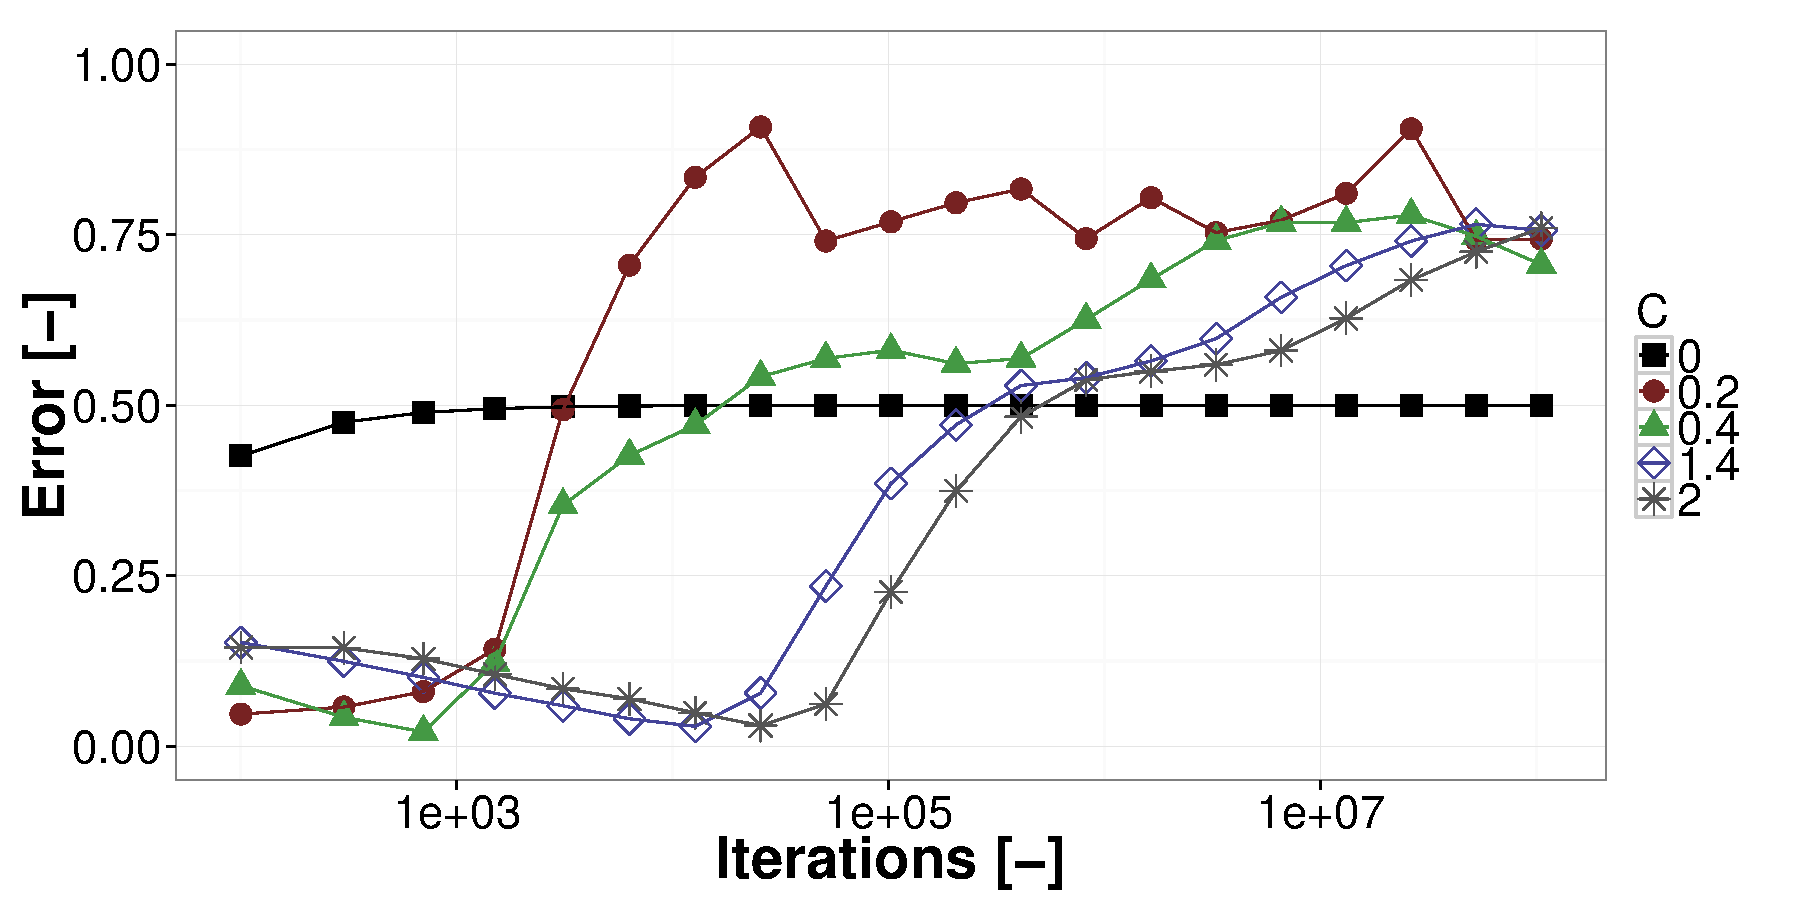
\includegraphics[width=0.55\textwidth]{figures/brps-MCTS-UCT.pdf} & 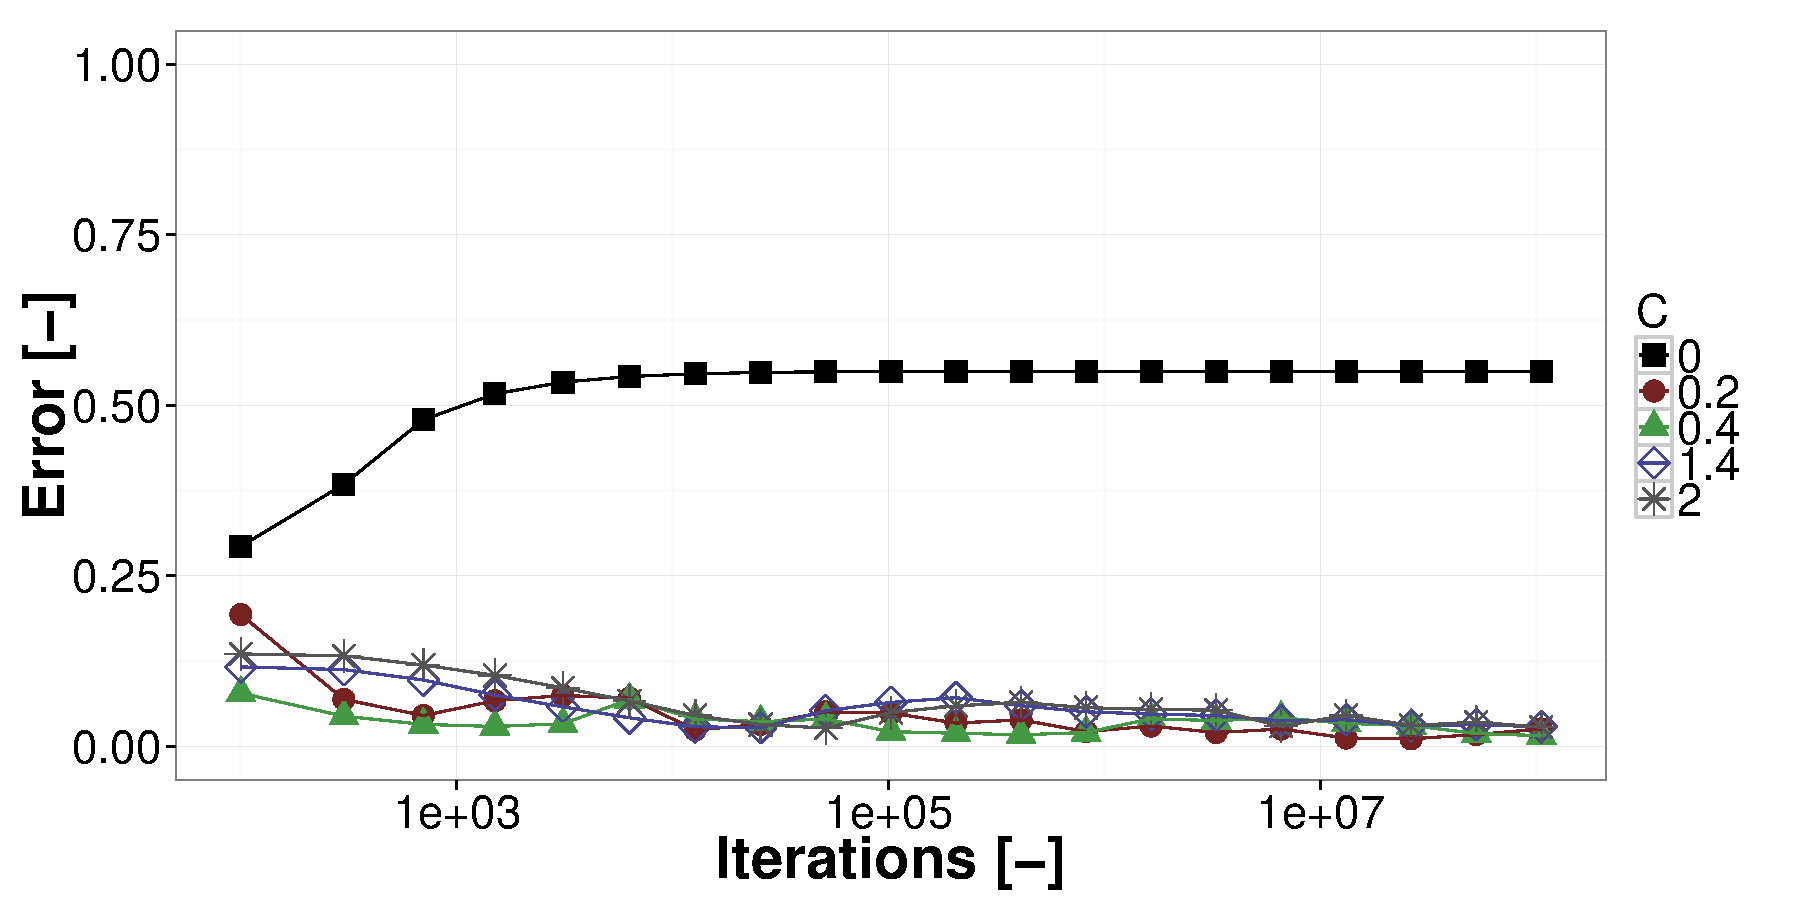
\includegraphics[width=0.55\textwidth]{figures/brps-MCTS-UCT-NONDET.pdf}\\
\hspace{-0.85cm}{\small MCTS-Exp3} & {\small MCTS-RM} \\
\hspace{-0.85cm}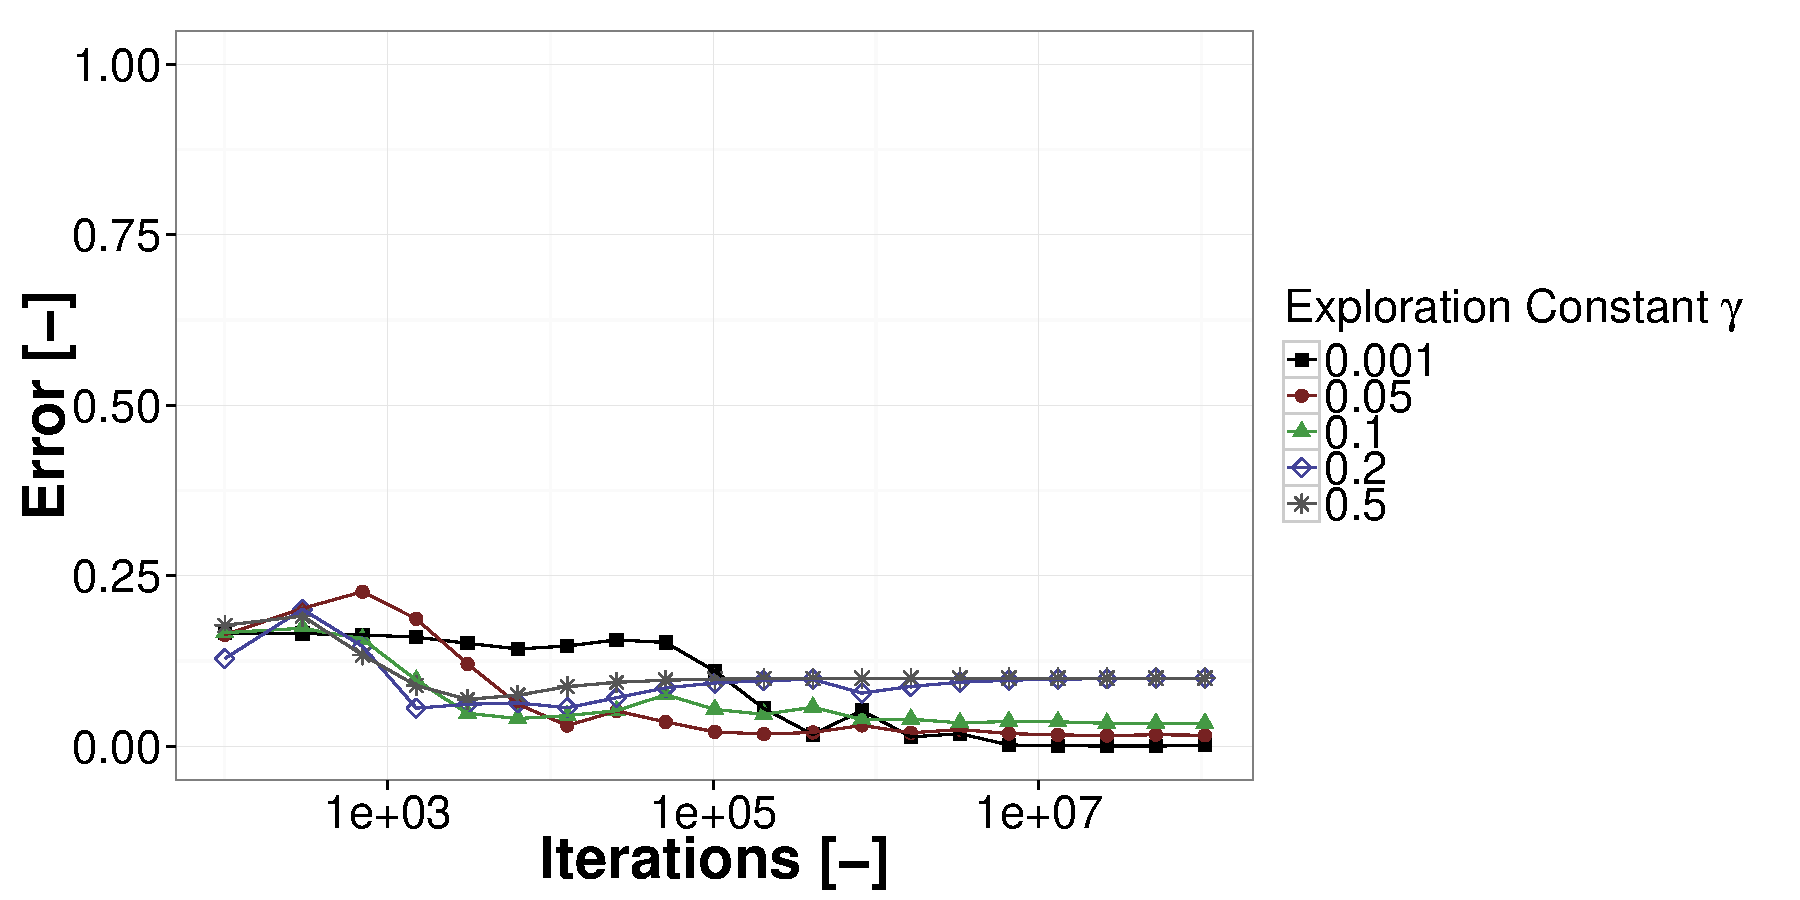
\includegraphics[width=0.55\textwidth]{figures/brps-MCTS-EXP3.pdf} & 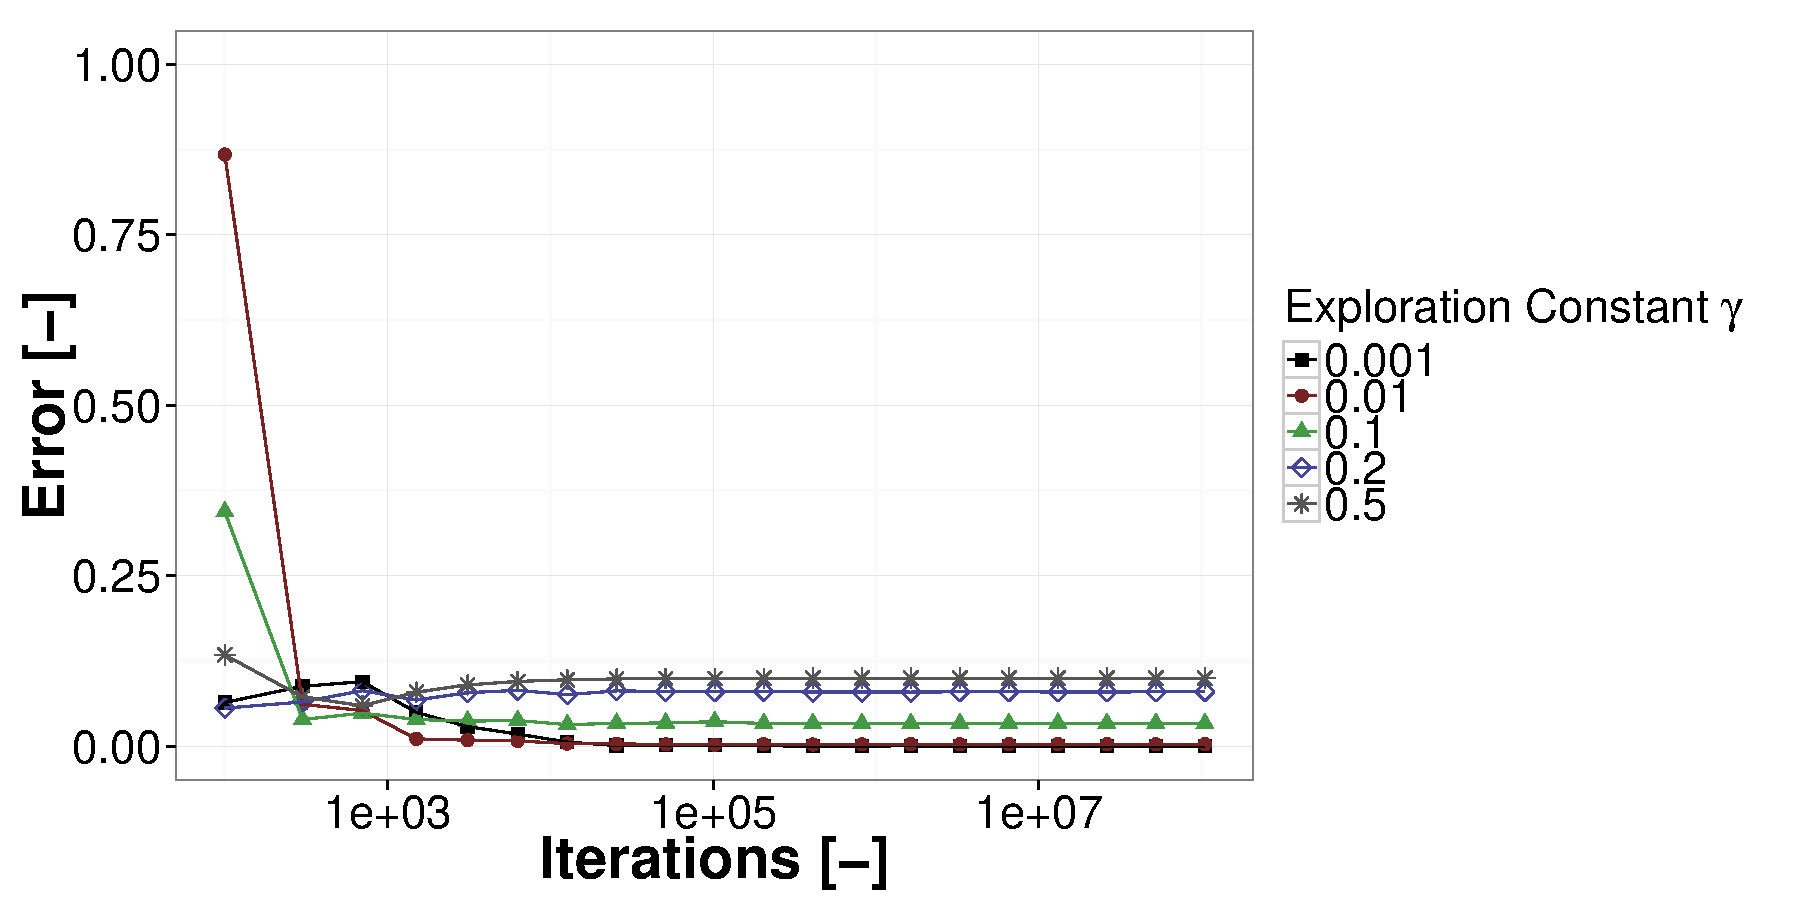
\includegraphics[width=0.55\textwidth]{figures/brps-MCTS-RM.pdf}
\end{tabular}
\caption{Exploitability of strategies of recommended by MCTS over time in Biased Rock, Paper, Scissors. Vertical axis represents exploitability. \label{fig:expl-brps}}
\end{figure}

The first observation is that UCT does not seem to converge to a low-exploitability strategy. The exploitability of the strategies of 
Exp3 and RM variants do converge to low-exploitability strategies, and the resulting approximation depend on the amount of exploration. 
If less exploration is used, then the resulting strategy is less exploitable, which is natural in the case of a single state. RM does seem to 
converge slightly faster than Exp3, as seen in the full simultaneous games as well. 

We then tried adding a stochastic tie-breaking rule to the UCT selection mechanism typically used in MCTS implementations, that chooses an 
action randomly when the scores of the best values are ``tied'' (less than $0.01$ apart).
One particularly striking observation is that this simple addition leads to a large drop in resulting exploitability, where exploitability
ranges from $[0.5,0.8]$ in the deterministic case, compared to $[0.01,0.05]$ with stochastic tie-breaking. 

\mlanctot{I noticed Vilo added his example to the SM-MCTS section so please modify this paragraph as necessary. Maybe it can be 
removed entirely?} We investigated this further and found a possible
explanation of this behavior. Consider the matrix game on the right of Figure~\ref{fig:egMatrixGames} in Section~\ref{sec:smg}.
Suppose DUCT is run on this game and players deterministically prefer the left-action. 
DUCT will always recieve rewards 0 and the exploration bias term will cause the players to round-robin over the actions indefinitely. 
However, each player can than improve by playing first action with probability 1. Breaking ties stochastically will lead the algorithm to 
discover the 1 and -1 rewards with high probability and allow the algorithm the break out or avoid this synchronization trap.

\subsection{Offline Equilibrium Computation}
We first compare the offline performance of the algorithm -- i.e., we measure overall computation time for each of the algorithms. 
The reported results are means of at least $30$ runs for each algorithm. 

\subsubsection{Goofspiel}
\begin{figure}
\centering
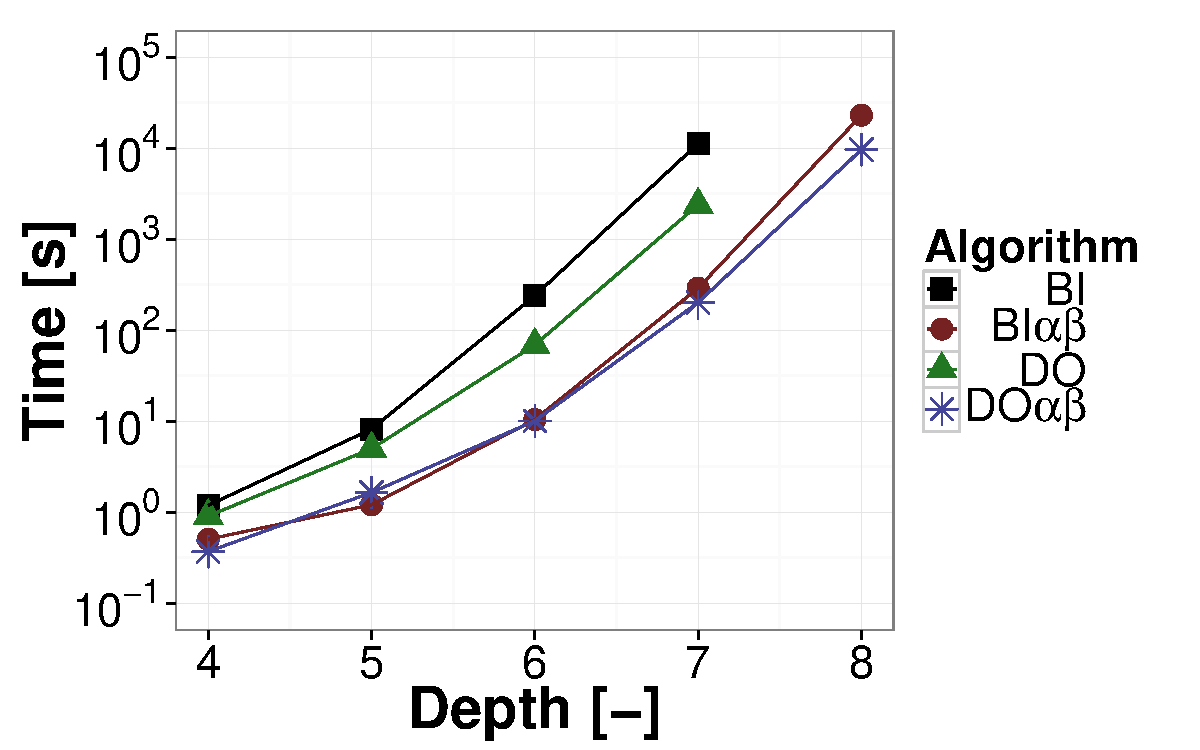
\includegraphics[width=0.5\textwidth]{figures/GS.pdf}
\caption{Comparison of running times on Goofspiel with increasing size of the deck.} \label{fig:off:res:gs}
\end{figure}

Figure~\ref{fig:off:res:gs} depicts the results for the card game Goofspiel (note the logarithmic y-scale).
The results show that a significant number of sub-games has a pure sub-game Nash equilibrium that can be computed using serialized alpha-beta algorithms.
Therefore, the performance of $\biab$ and $\doab$ is fairly similar and the gap only slowly increases in favor of $\doab$ with the increasing size of the game.
Both of these algorithms significantly reduce the number of states visited by the backward induction algorithm (i.e., excluding the number of states evaluated by serialized alpha-beta algorithm).
While \textsc{BI} algorithm evaluates on average more than $32\cdot10^6$ nodes in the setting with $7$ cards in more than $3$ hours, $\biab$ evaluates only $198986$ nodes in less than $5$ minutes. 
The performance is further improved by $\doab$ that evaluates on average $51035$ nodes in less than $4$ minutes.
However, the overhead of the algorithm is slightly higher in case of $\doab$; hence, the difference between $\doab$ and $\biab$ is relatively small in this case.
Finally, the results show that even simple \textsc{DO} algorithm without serialized alpha-beta search can improves the performance of \textsc{BI}.
In the setting with $7$ cards, \textsc{DO} evaluates more than $6\cdot10^6$ nodes which takes on average almost 40 minutes.

The results on Goofspiel highly contrast with the Goofspiel results of the pruning algorithm SMAB presented in \cite{Saffidine12SMAB}.
In their work, the number of evaluated nodes was at best around $20\%$, and the running time improvement was only marginal. 

\begin{figure}
\centering
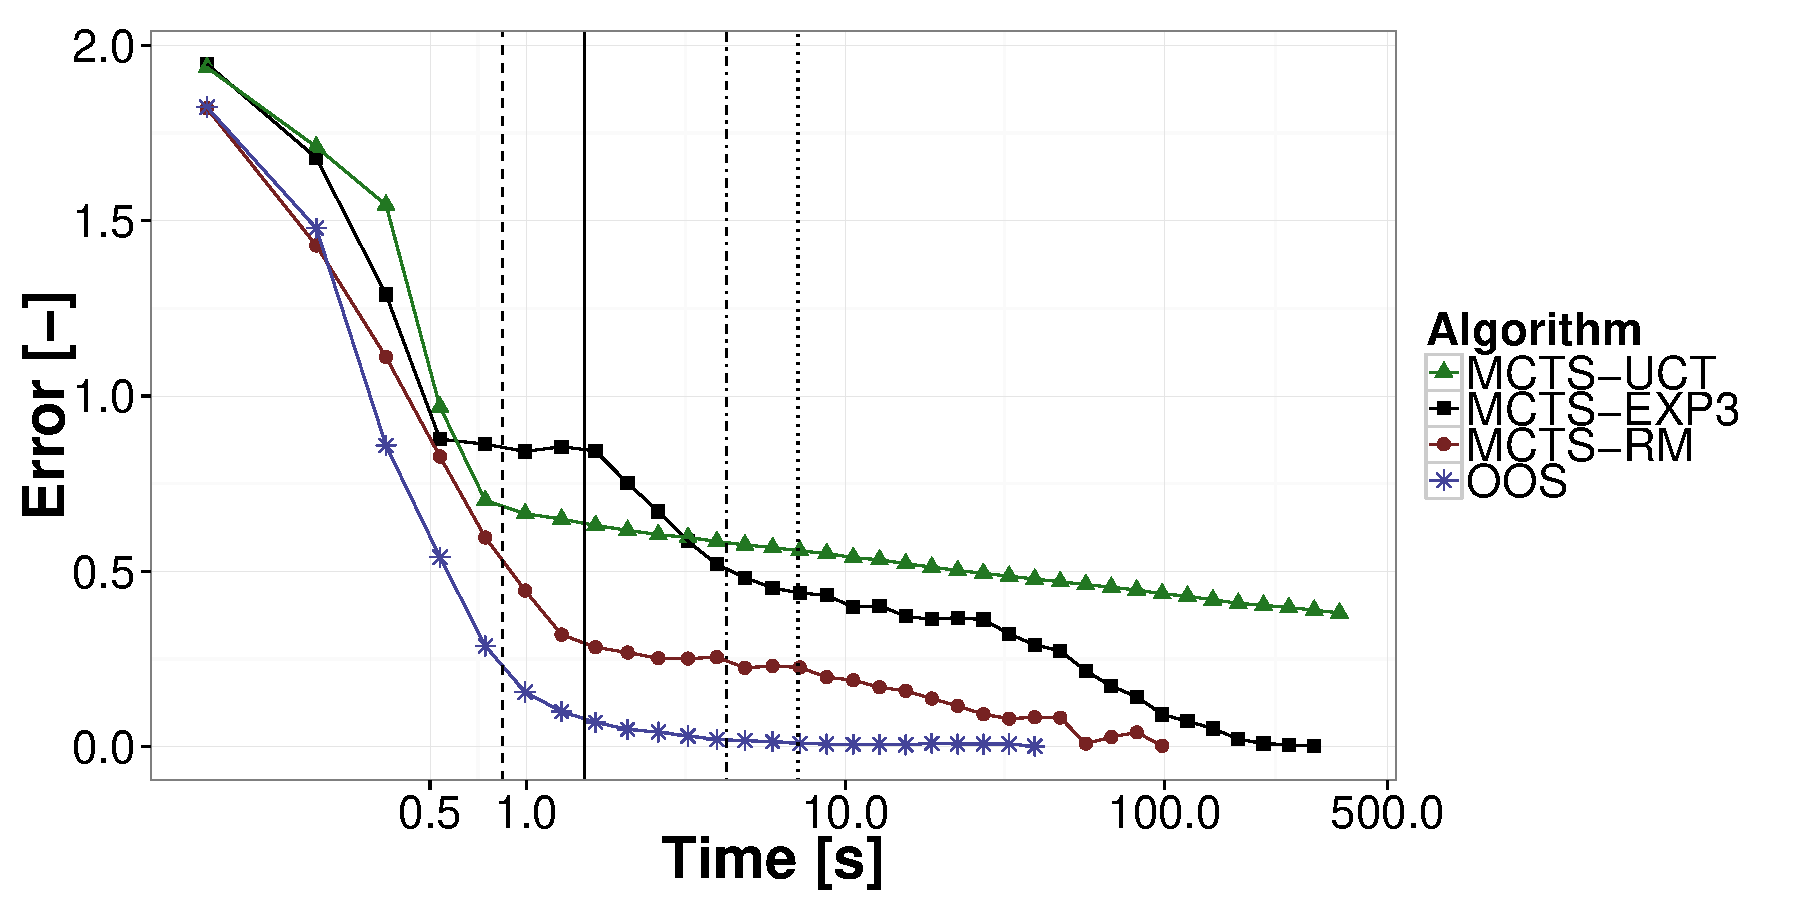
\includegraphics[width=0.85\textwidth]{figures/convergence-gs.pdf}
\caption{Convergence comparison of different sampling algorithms on Goofspiel with $5$ cards. The vertical lines correspond to computation times for exact algorithms.} \label{fig:off:conv:gs}
\end{figure}

Next we focus on the convergence of sampling algorithms -- i.e., their ability to approximate Nash equilibrium strategies of the complete game. 
Figure~\ref{fig:off:conv:gs} depicts the results in this offline settings for Goofspiel game with $5$ cards (note the logarithmic x-scale).
We compare MCTS algorithms with three different selection functions (UCT, EXP3, and RM), and OOS algorithm. 
The results are means out of $20$ runs of each algorithm.
The results show that OOS is the fastest out of all sampling algorithms during the whole time. 
MCTS with Regret Matching selection function is only slightly slower, however, other two selection functions perform worse. 
While EXP3 eventually converges close to $0$, the exploitability of UCT decreases rather slowly and it was still over $0.35$ at the time limit of $300$ seconds. 
These results confirm theoretical properties for the algorithms, where it can be quite slow for EXP3 and UCT.
Moreover, when we have not used randomization in UCT, the algorithm was not able to converge to error lower than $0.5$ in the time limit. 
On the other hand, both OOS and RM confirm their quick convergence, witch is aligned with previous existing results~\cite{Lanctot13Goofspiel}.
The vertical lines represent times for exact algorithms.
In Goofspiel $5$, $\biab$ is slightly faster and finishes first in less than $1$ second, following by $\doab$ ($1.52$ seconds), \textsc{DO} ($4.25$ seconds), and \textsc{BI} ($7.11$).


\subsubsection{Pursuit-Evasion Games}
\begin{figure}
\centering
	\begin{subfigure}{0.49\textwidth}
		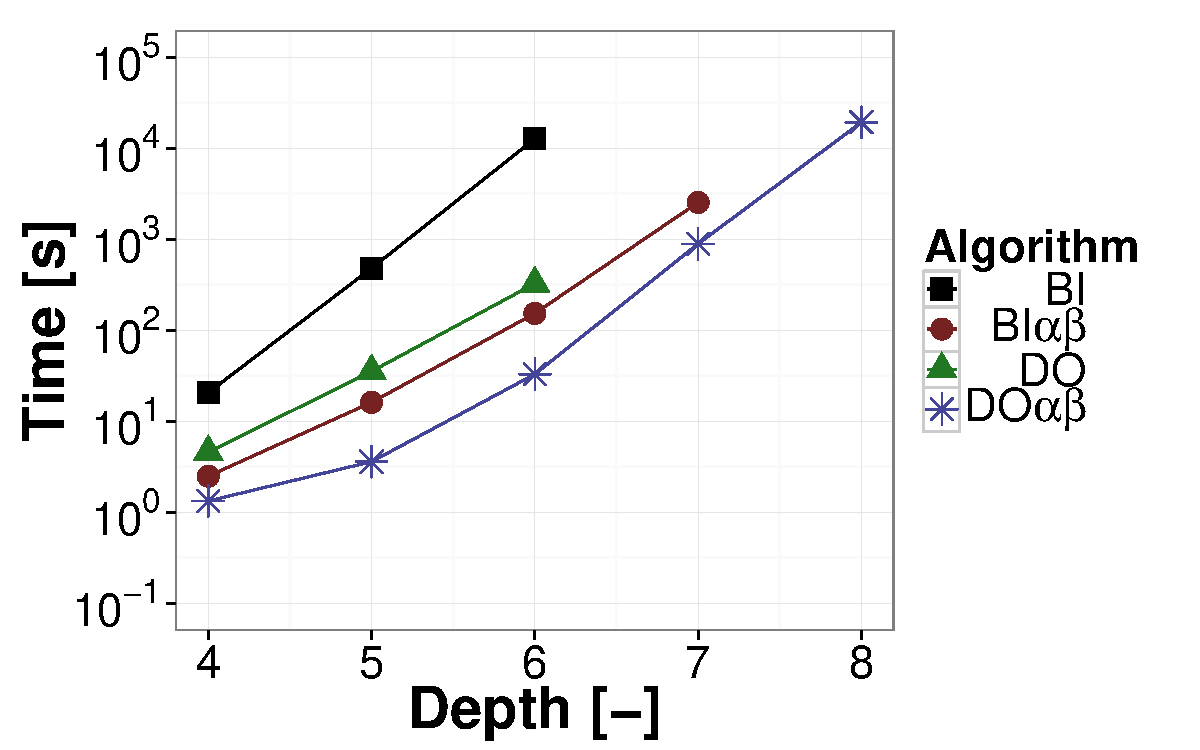
\includegraphics[width=1\textwidth]{figures/PEG4x4.pdf}\caption{}\label{fig:off:res:peg4}
	\end{subfigure}
	\begin{subfigure}{0.49\textwidth}
		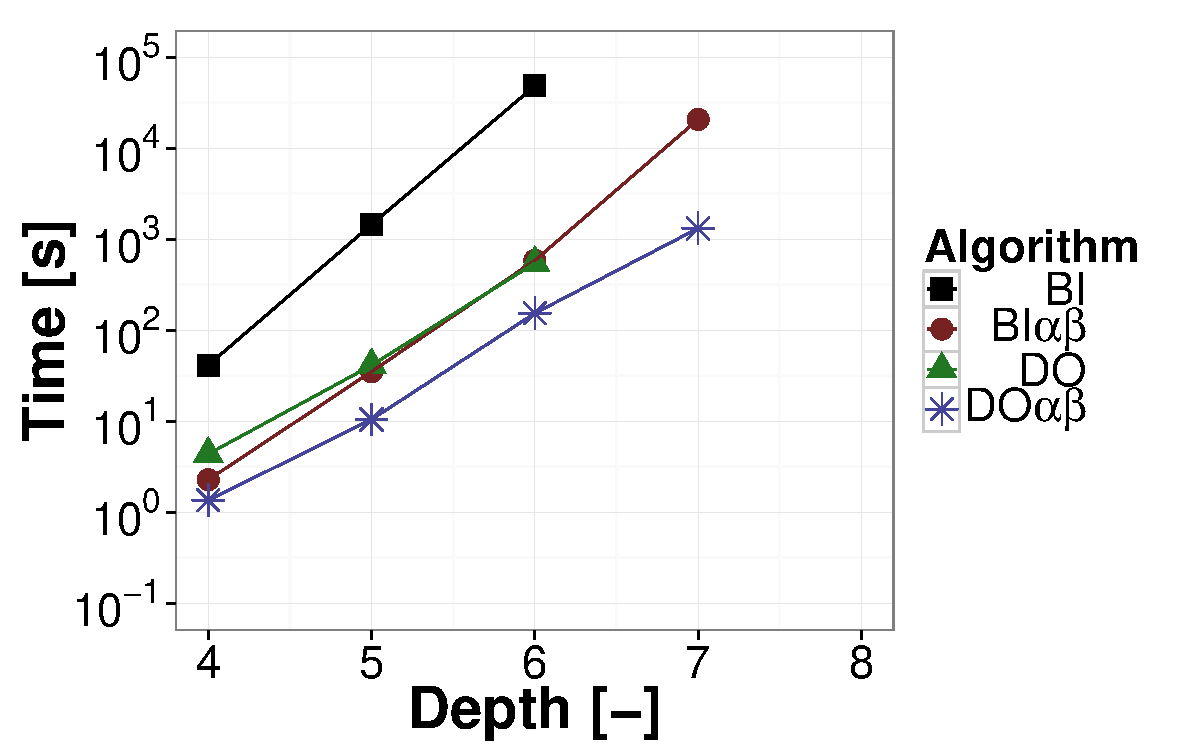
\includegraphics[width=1\textwidth]{figures/PEG5x5.pdf}\caption{}\label{fig:off:res:peg5}
	\end{subfigure}
\caption{Comparison of running times on pursuit-evasion game with increasing number of moves: sub-figure (a) depicts the results on $4\times4$ grid graph, (b) depicts results for $5\times5$ grid.} \label{fig:off:res:peg}
\end{figure}

The results on pursuit-evasion games show more significant improvement when comparing $\doab$ and $\biab$ (see Figure~\ref{fig:off:res:peg}). In all settings, the $\doab$ is significantly the fastest. When we compare the performance on graph $5\times5$ with depth set to $6$, \textsc{BI} evaluates more than $49\cdot10^6$ nodes that takes more than $13$ hours. On the other hand, $\biab$ evaluates on average $42001$ nodes taking almost $10$ minutes ($584$ seconds). Interestingly, the benefits of pure integration with alpha-beta search is not that helpful in this game.
This is apparent from results of \textsc{DO} algorithm that evaluates less than $2\cdot10^6$ nodes but it takes slightly over $9$ minutes on average ($547$ seconds). Finally, $\doab$ evaluates only $6692$ nodes and it takes the algorithm less than $3$ minutes.

Large parts of pursuit-evasion game can be solved by serialized alpha-beta algorithms.
These parts typically corresponds to clearly winning, or clearly loosing positions for a player.
However, since there are only two pursuit units, it is still necessary to use mixed strategies for final coordination (capturing the evader close to edge of the graph), and thus mixing strategy occurs near the end of the game tree. 
Therefore, serialized alpha-beta is not able to solve all sub-games, while double-oracle provides additional pruning and cause the improvement in computation time for $\doab$ compared to $\biab$ and all the other algorithms.

\begin{figure}
\centering
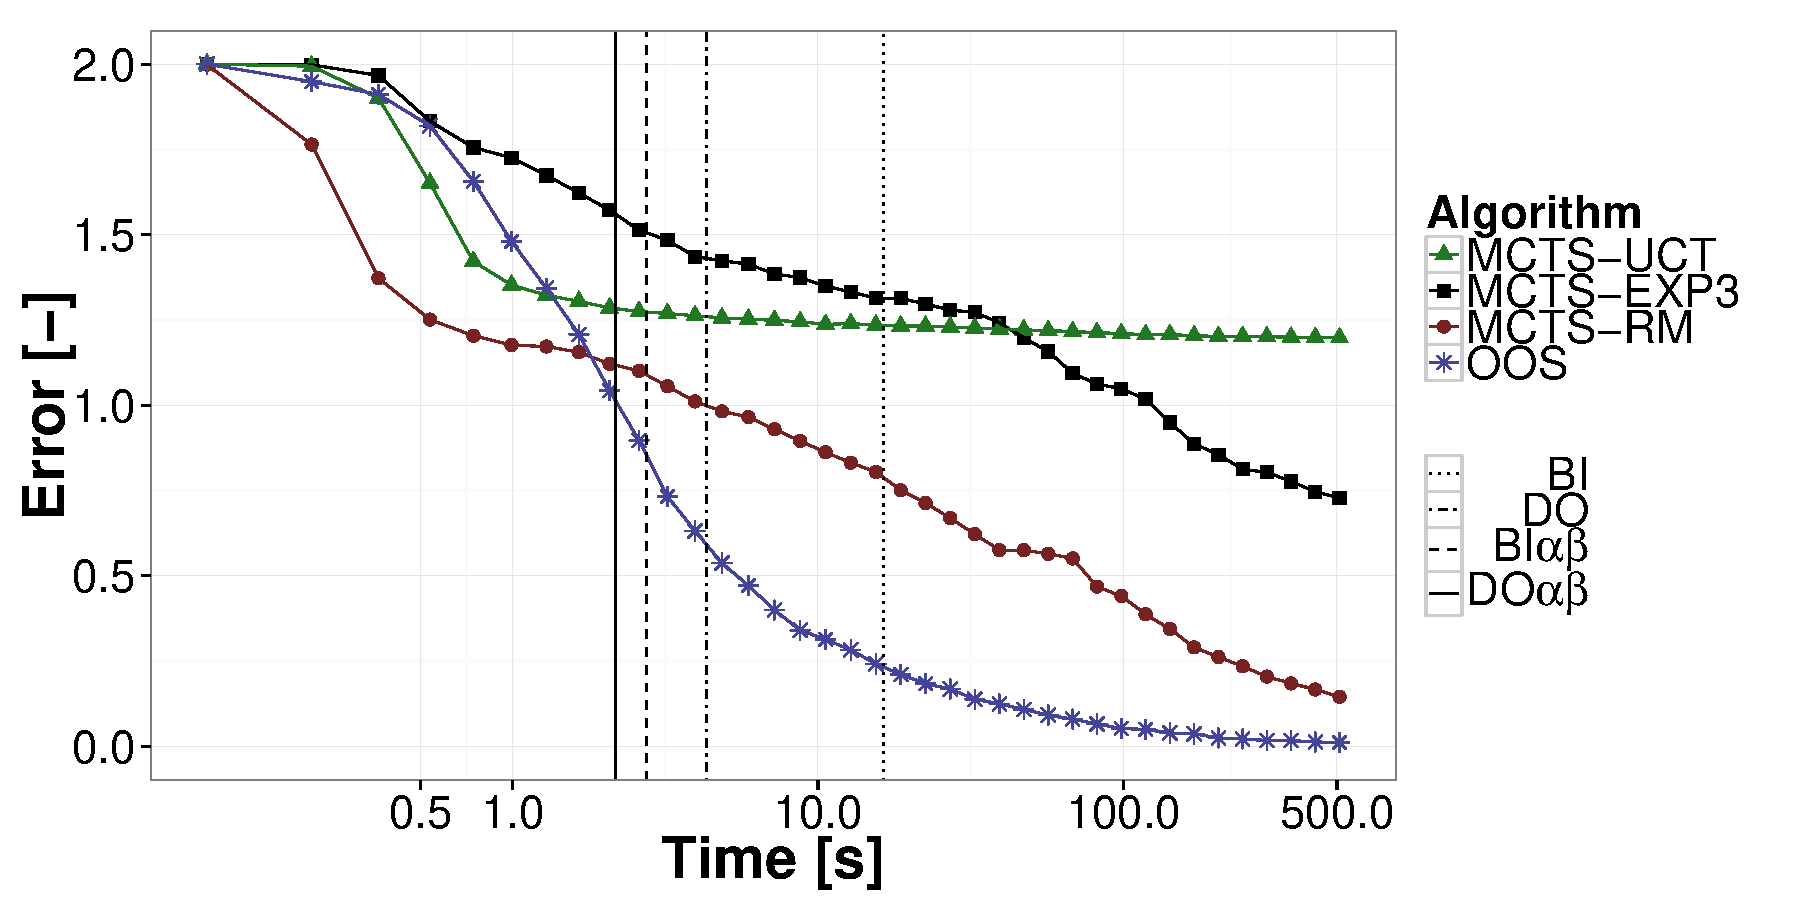
\includegraphics[width=0.85\textwidth]{figures/convergence-peg.pdf}
\caption{Convergence comparison of different sampling algorithms on pursuit-evasion game, on $4\times4$ graph, with depth set to $4$. The vertical lines correspond to computation times for exact algorithms.} \label{fig:off:conv:peg}
\end{figure}

We turn to convergence of the sampling algorithms.
The results are depicted in Figure~\ref{fig:off:conv:peg} for the smaller $4\times4$ graph and $4$ number of moves for each player (note again the logarithmic y-scale).
The starting positions were selected such that there does not exist a pure NE strategy in the game.
The results again show that OOS is overall the fastest out of all sampling algorithms, however, during the first iterations both UCT and RM are faster and their exploitability is smaller. 
On the other hand, while OOS is able to keep the convergence rate and reach almost $0$ exploitability, UCT again converges to an exploitable strategy with error $1.16$ at best in the time limit of $500$ seconds.
The convergence of RM is much better, however the best final error is $0.14$ in the given time.
Finally, EXP3 converges even more slowly compared to the Goofspiel.
The main difference between the games is the size of the branching factor for the second player (pursuer controls two simultaneously moving units), which can cause more difficulties for the sampling algorithms to estimate good strategies.

As before, the vertical lines represent times for exact algorithms.
In pursuit-evasion game of this setting, $\doab$ is slightly faster and finishes first in $2.77$ seconds, following by $\biab$ ($2.89$ seconds), \textsc{DO} ($5.48$ seconds), and \textsc{BI} ($12.5$).

\subsubsection{Oshi-Zumo}
\begin{figure}
\centering
	\begin{subfigure}{0.49\textwidth}
		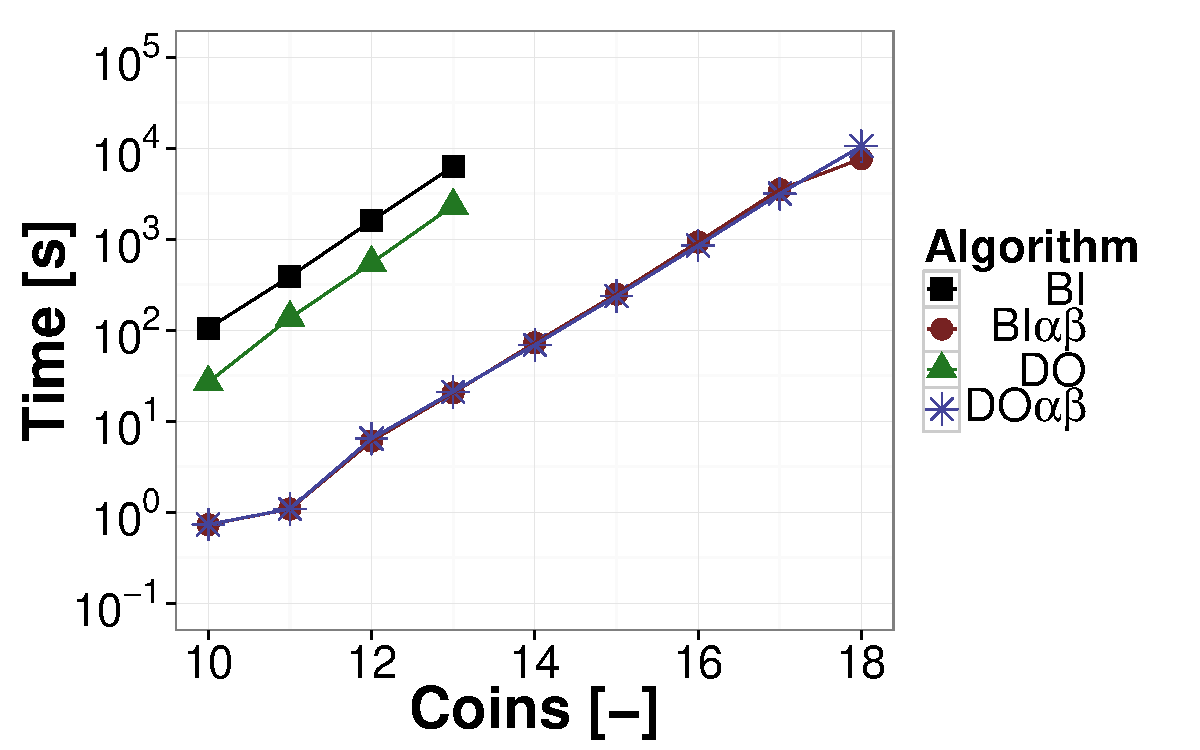
\includegraphics[width=1\textwidth]{figures/OZ-K3.pdf}\caption{}\label{fig:off:res:oz3}
	\end{subfigure}
	\begin{subfigure}{0.49\textwidth}
		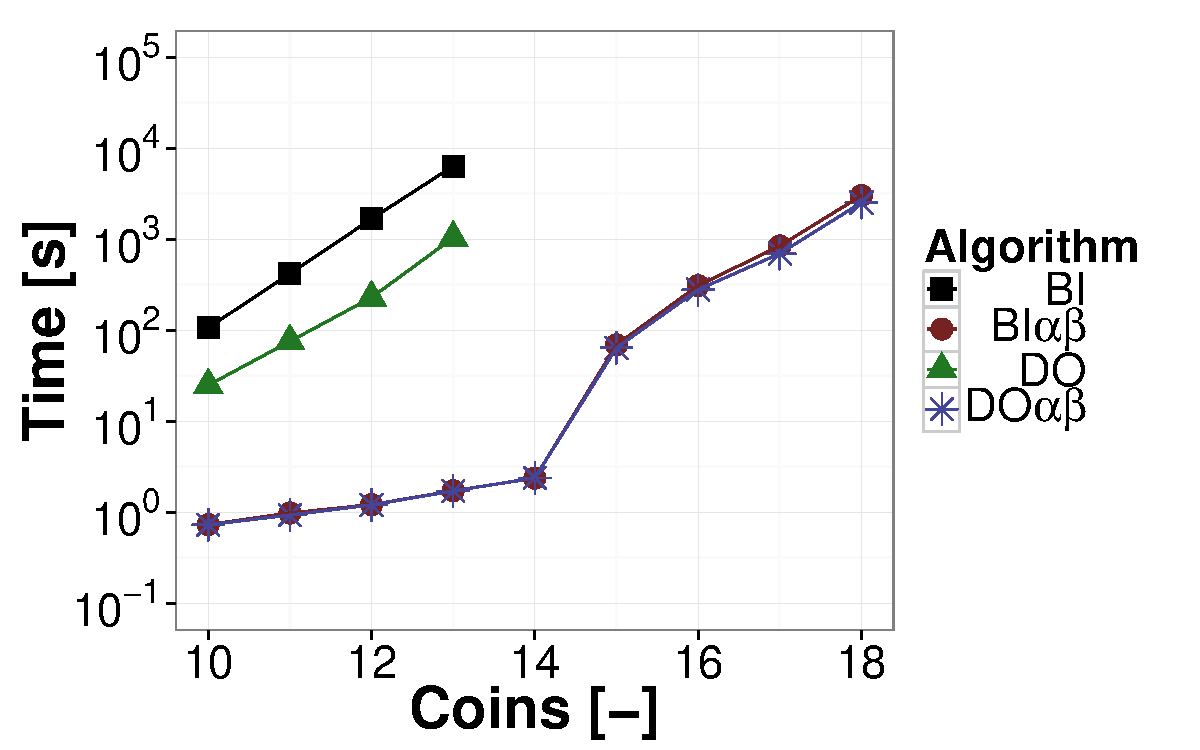
\includegraphics[width=1\textwidth]{figures/OZ-K4.pdf}\caption{}\label{fig:off:res:oz4}
	\end{subfigure}
\caption{Comparison of running times on the Oshi-Zumo game with increasing number of coins: sub-figure (a) depicts the results on with $K$ set to $3$, (b) depicts the results with $K=4$.} \label{fig:off:res:oz}
\end{figure}

Many instances of the Oshi-Zumo game have Nash equilibria in pure strategies. 
Although this does not hold for all the instances, the size of the sub-games with pure NE are rather large and cause dramatic computation speed-up for both algorithms using serialized alpha-beta search.
If the game does not have equilibria in pure strategies, the mixed strategies are still required only near the root node and large end-games are solved using alpha-beta search.
Note that this is different to pursuit-evasion games, where mixed strategies were necessary close to the end of the game tree.
Figure~\ref{fig:off:res:oz} depicts the results for two different setting of the playing field $K$ is either set to $3$ or $4$.
In both cases, the graphs clearly highlights when the whole game does not have an equilibrium in pure strategies -- for $K$ equal to $3$, the change occurs when the number of coins increase from $11$ to $12$, for $K=4$ the first setting with non-pure equilibria is in case with $15$ coins for each player.

The consequence of the advantage of $\biab$ and $\doab$ algorithms that exploit serialized variants of alpha-beta algorihtms is dramatic in Oshi-Zumo game. 
We can see that both \textsc{BI} and \textsc{DO} scale rather badly.
The algorithms were able to scale up to $13$ coins in reasonable time. 
For setting with $K=4$ and $13$ coins, it takes almost $2$ hours for \textsc{BI} to solve the game (the algorithm evaluates $15\cdot10^6$ nodes).
\textsc{DO} improves the performance slightly (the algorithm evaluates nearly $6\cdot10^6$ nodes in $40$ minutes), however, the difference between alpha-beta algorithm is dramatic. 
Both $\biab$ and $\doab$ are in essence solved by executing a single alpha-beta search on each serialization.
Therefore, their performance is identical and it takes $21$ seconds to solve the game.
With an increasing number of coins the algorithms need to find mixed Nash equilibria, however, their performance is in both cases very similar.

\begin{figure}
\centering
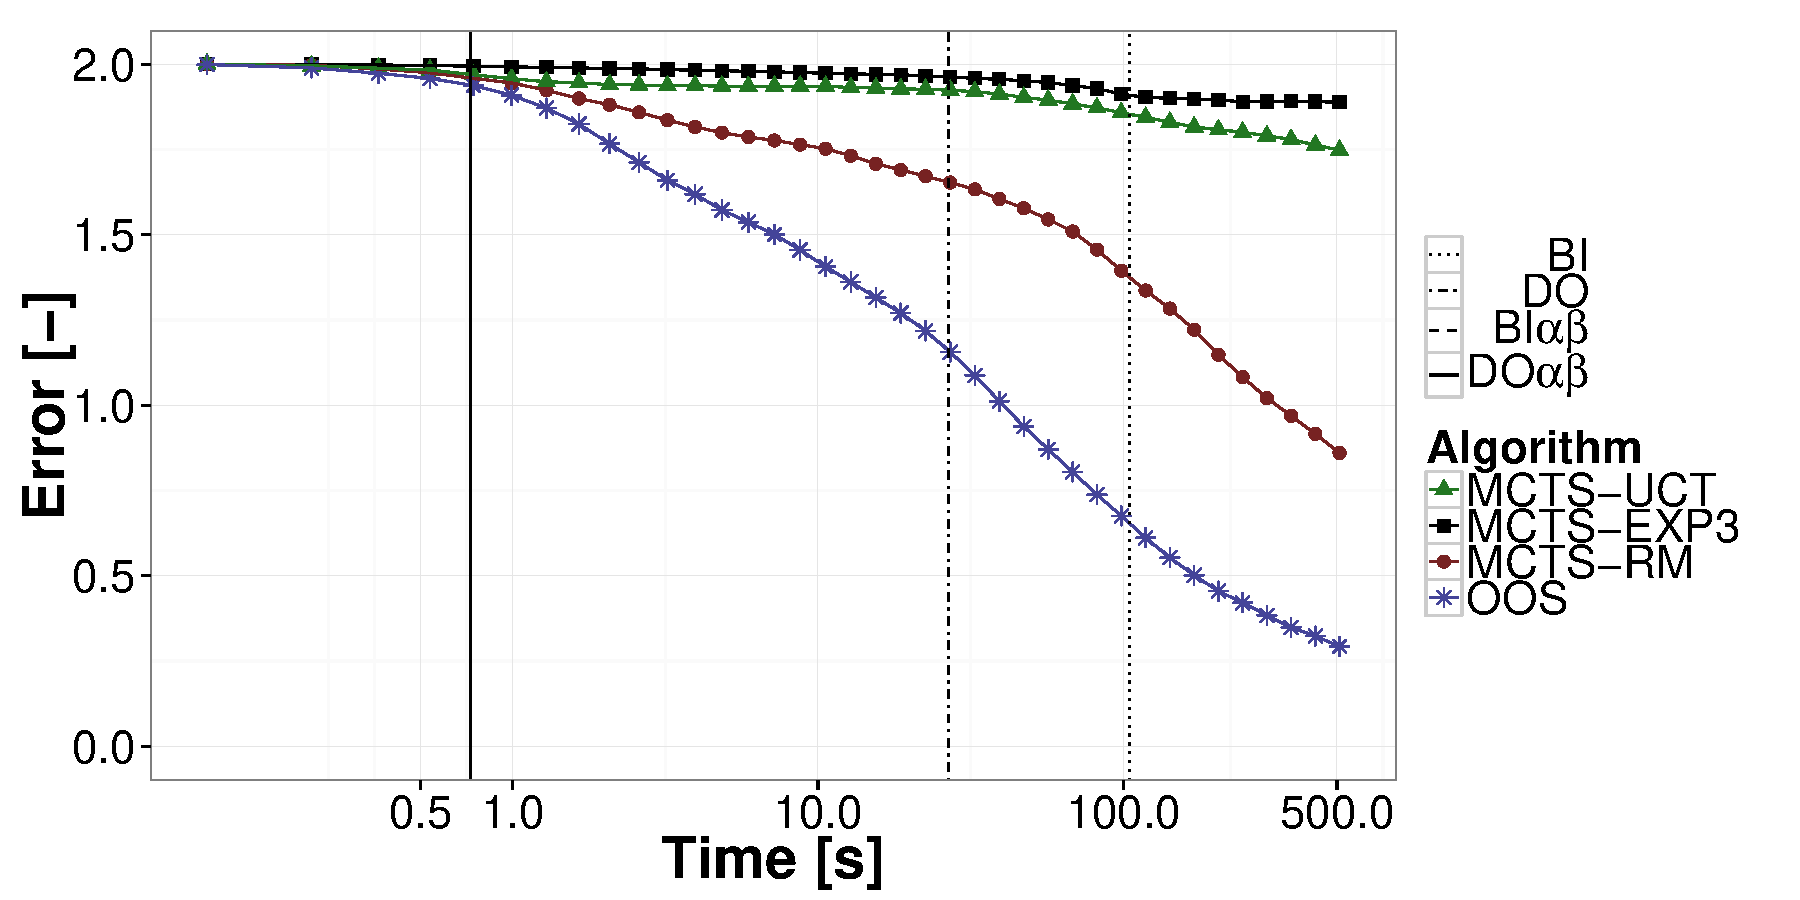
\includegraphics[width=0.85\textwidth]{figures/convergence-oz.pdf}
\caption{Convergence comparison of different sampling algorithms on Oshi-Zumo game, with $10$ coins, $K=3$, and $M=1$. The vertical lines correspond to computation times for exact algorithms.} \label{fig:off:conv:oz}
\end{figure}

Figure~\ref{fig:off:conv:oz} depicts results for convergence of the sampling algorithms for the game with $10$ coins, $K$ set to $3$ and minimum bid set to $1$. This is an easy game for $\doab$ and $\biab$ with pure strategy and both of these algorithms are able to solve the game in less than a second ($0.73$). However, due to large branching factor for both players ($10$ actions at the root node for each player) all sampling algorithms converge extremely slowly. Again, OOS is the best one, however, in a given time limit ($500$ seconds) the algorithm converged to error slightly below $0.5$ ($0.41$). On the other hand, all of the other sampling algorithms perform significantly worse -- RM ends with error slightly over $1$, UCT with $1.50$, and EXP3 with $1.88$.
This confirms our findings from the previous experiment that increasing branching factor slows down the convergence rate.
Secondly, since there is a pure Nash equilibrium in this particular game configuration, the convergence of the algorithms is also slower since they essentially mix the strategy during the iterations in order to explore the unvisited parts of the game tree. Since none of the sampling algorithms can directly exploit this fact, their performance in offline solving games like Oshi-Zumo is not compelling. On the other hand, the existence of pure NE explains the better performance of UCT compared to EXP3 that is forced to explore more broadly.

\subsubsection{Random Games}
In the first variant of the randomly generated games we used games with utility values randomly drawn from a uniform distribution $[0,1]$. 
Such games represent an extreme case, where neither alpha-beta search, nor double-oracle algorithm can save much computation time, since each action can lead to arbitrarily good or bad terminal state. 
In these games, \textsc{BI} algorithm is typically the fastest.
Even though both $\biab$ and $\doab$ evaluate marginally less nodes ($\approx90\%$), the overhead of the algorithms (repeated calculation of alpha-beta algorithm, repeatedly solving linear programs, etc.) causes slower runtime performance in this case.

However, completely random games are rarely instances that do not need to be solved in practice.
The situation changes, when we use the intuition of good and bad moves and thus add correlation to the utility values.
Figure~\ref{fig:off:res:rg} depicts the results for two different branching factors $4$ and $5$ for each player and increasing depth.
The results show that $\doab$ outperforms all remaining algorithms, although the difference is rather small (still statistically significant).
On the other hand, \textsc{DO} without serialized alpha-beta is not able to outperform \textsc{BI}. 
This is most likely caused by a larger support in mixed sub-game equilibria that cause enumerating most of the actions by the double-oracle algorithm. 
Moreover, this is also demonstrated by the performance of $\biab$ that is only slightly better compared to \textsc{BI}.

The fact that serialized alpha-beta is less successful in randomly generated games is noticeable also when comparing the number of evaluated nodes.
For case with branching factor set to $4$ for both players, and depth $7$, \textsc{BI} evaluates almost $18\cdot10^6$ nodes in almost $3.5$ hours, while $\biab$ evaluates more than $\approx10\cdot10^6$ nodes in almost $3$ hours. 
\textsc{DO} evaluates even more nodes compared to $\biab$ ($\approx12\cdot10^6$) and it is slower compared to both \textsc{BI} and $\biab$. 
Finally, $\doab$ evaluates $\approx2\cdot10^6$ nodes on average and it takes the algorithm slightly over $80$ minutes.

\begin{figure}
\centering
	\begin{subfigure}{0.49\textwidth}
		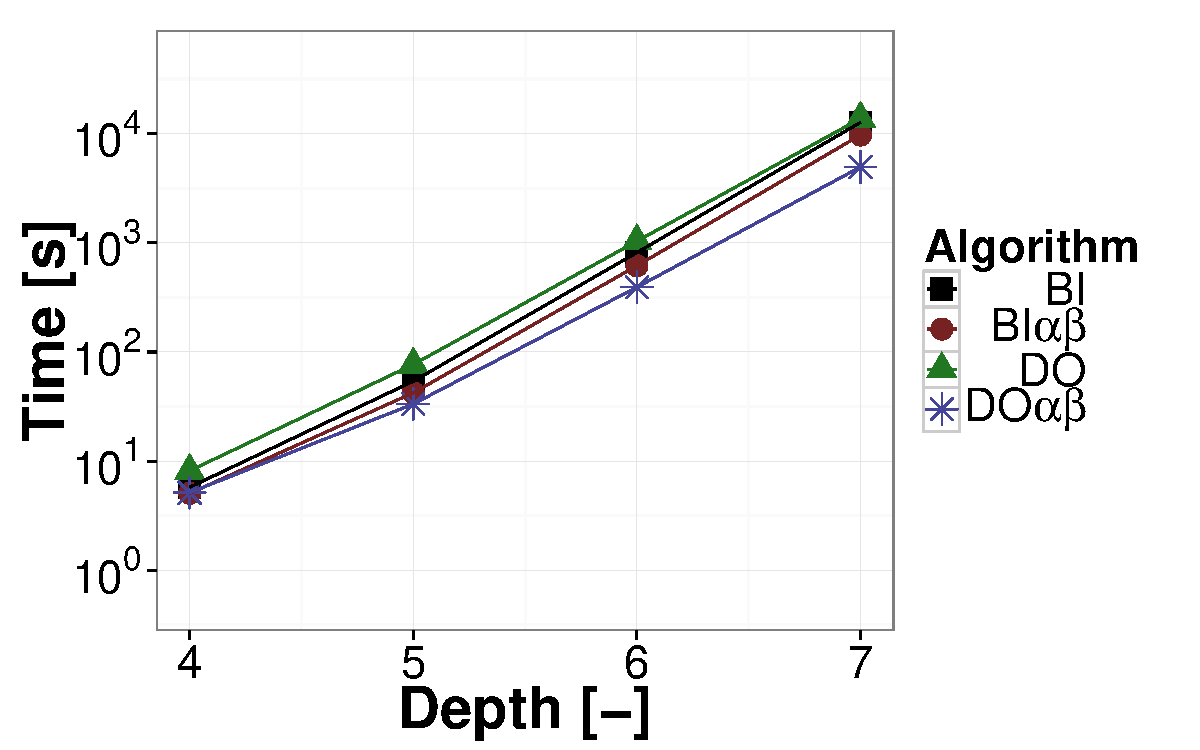
\includegraphics[width=1\textwidth]{figures/RG-BF4-BIN-FALSE.pdf}\caption{}\label{fig:off:res:rgbf4}
	\end{subfigure}
	\begin{subfigure}{0.49\textwidth}
		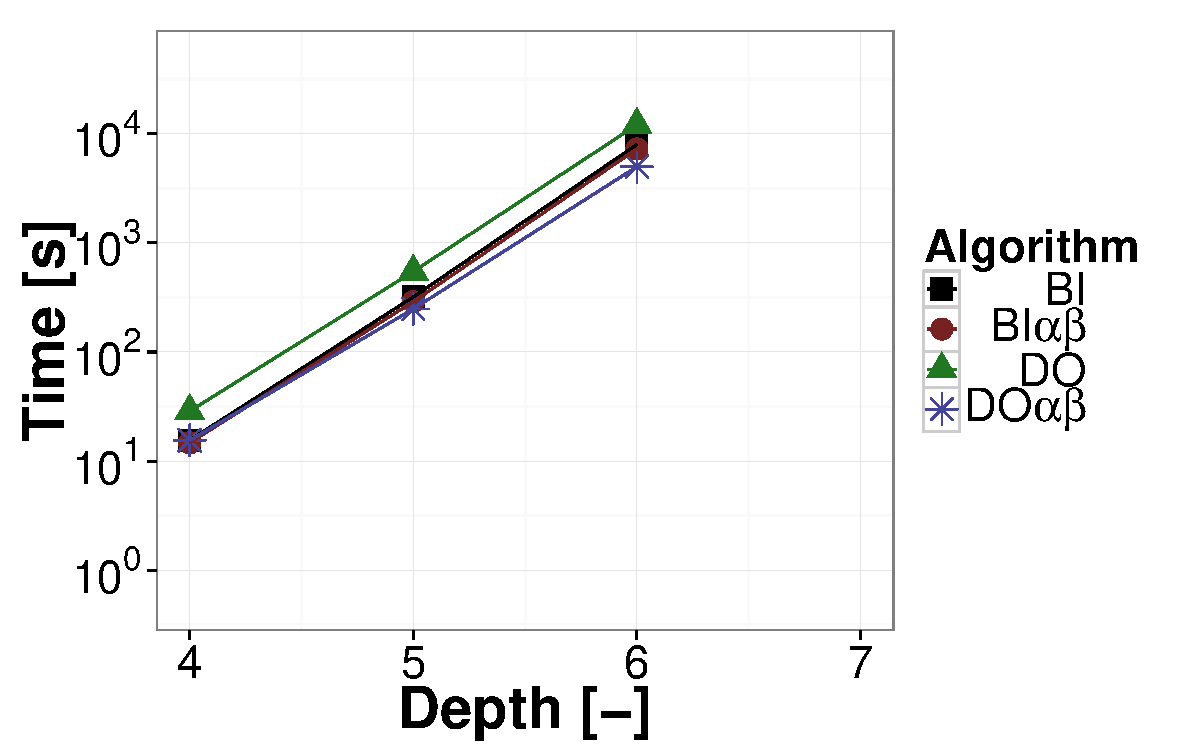
\includegraphics[width=1\textwidth]{figures/RG-BF5-BIN-FALSE.pdf}\caption{}\label{fig:off:res:rgbf5}
	\end{subfigure}
\caption{Comparison of running times on randomly generated games with increasing depth: sub-figure (a) depicts the results with branching factor set to $4$ actions for each player, (b) depicts the results with branching factor $5$.} \label{fig:off:res:rg}
\end{figure}

\begin{figure}
\centering
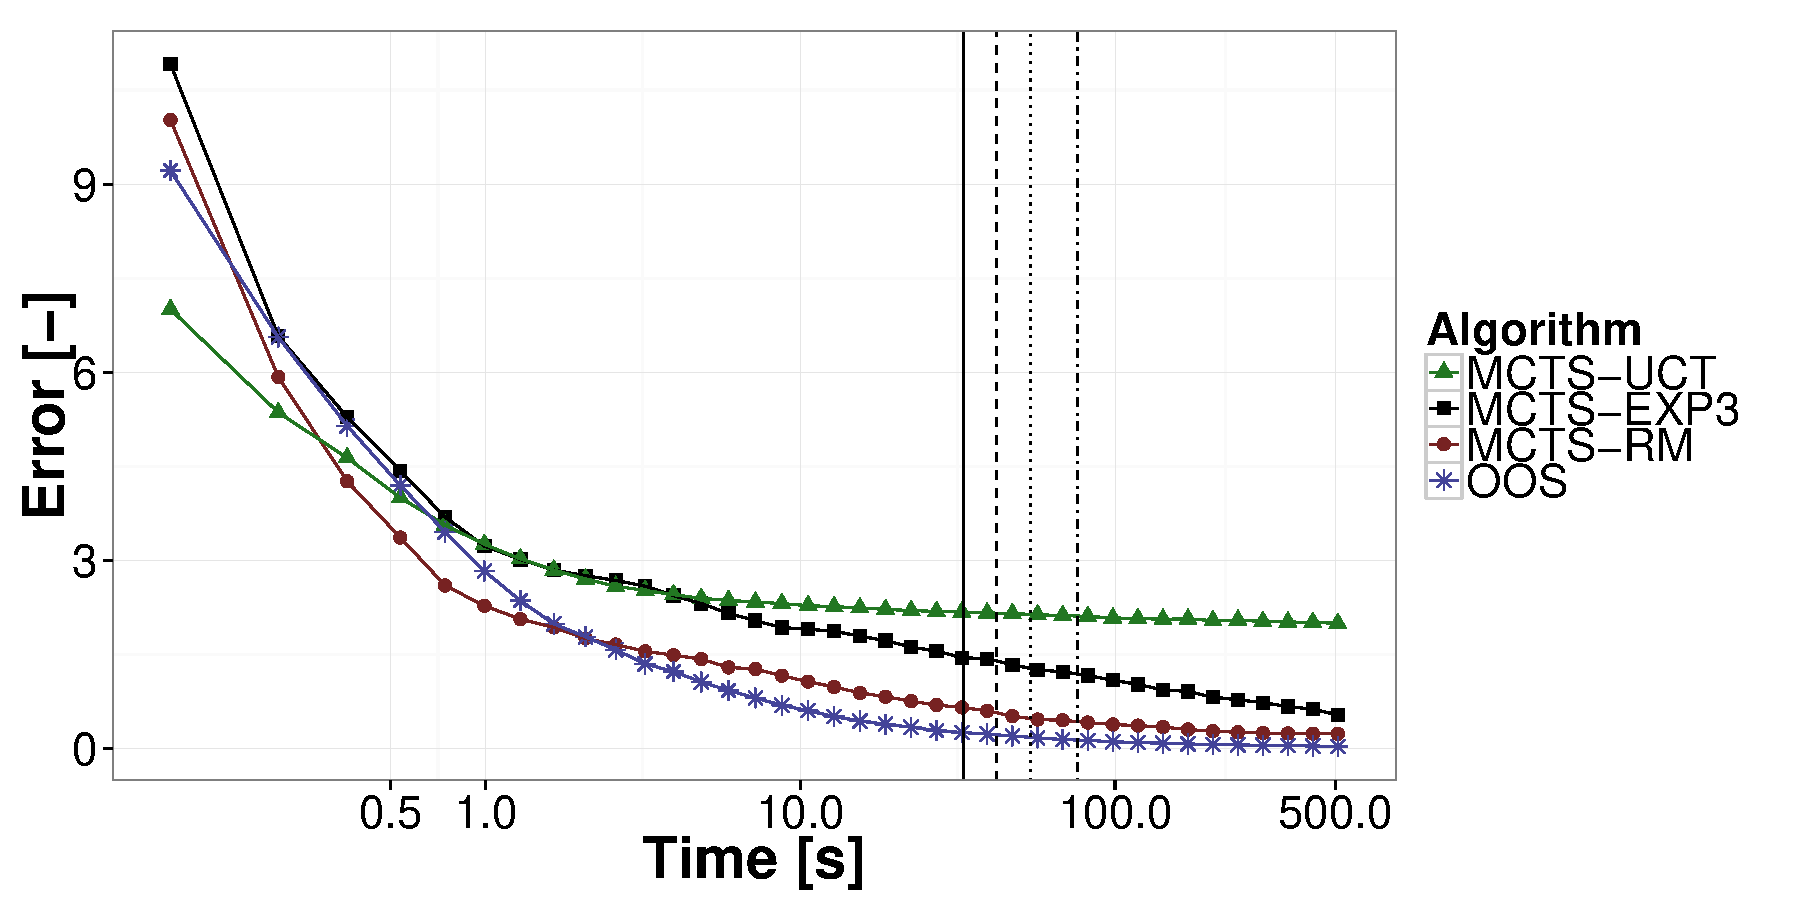
\includegraphics[width=0.85\textwidth]{figures/convergence-rg-fix.pdf}
\caption{Convergence comparison of different sampling algorithms on random game with branching factor $4$ and depth $5$. The vertical lines correspond to computation times for exact algorithms.} \label{fig:off:conv:rg}
\end{figure}

Figure~\ref{fig:off:conv:rg} depicts the results for convergence of the sampling algorithms for the random game with correlated utility values, branching factor set to $4$ and depth $5$. Interestingly, there is a much less difference between the performance of the sampling algorithms in this game. Since these games are generally more mixed (i.e., NE require to use mixed strategies in many states of the game), they are much more suitable for the sampling algorithms. In the overall performance, again OOS is the winner, however, the performance of RM is very similar and even better during the first second. Again, since the game is more mixed, EXP3 outperforms UCT in the longer run, however, it is the worst sampling algorithm during the first iterations.

\subsubsection{Tron}
When comparing the exact algorithms on offline computation, the results are affected by the fact that pure NE exists in all smaller instances.
Therefore, the performance of $\biab$ and $\doab$ is essentially the same since serialized alpha-beta is able to solve the game. Moreover, the performance of standard BI is very weak, since the size of the game increases dramatically with increasing size of the grid (the longest branch of the game tree has $\left(0.5\cdot w\cdot l - 1\right)$ joint actions, where $w$ and $l$ are dimensions of the grid). While BI is able to solve the grid $5\times6$ in $143$ seconds, it takes almost $30$ minutes to solve $6\times6$ grid. The same instance takes $\biab$ and $\doab$ $1.5$ seconds, however, the size of the game tree quickly prohibits the algorithms from computing the exact solution -- both algorithms solved at most the grid of size $8\times8$ that takes $25$ minutes to solve. 

The size of the game tree in Tron also causes slow convergence for sampling algorithms.
Figure~\ref{fig:off:conv:tron} depicts the results for the grid $5\times6$.
Consistently with the previous results, OOS performs the best and it is able to converge to very close to exact solution in $300$ seconds. 
Similarly, both RM and EXP3 are again eventually able to converge to a very small error, however, it take them more time and in the time limit they achieve error $0.05$, or $0.02$ respectively. 
Finally, UCT performs reasonably good during the first $10$ seconds, where the exploitability is better than both RM and EXP3. 
This is most likely due to existence pure NE, however, the length of the game tree prohibits UCT to converge and the best error the algorithm was able to achieve in the time limit was equal to $0.68$.

\subsubsection{Discussion}
The offline comparison of the algorithms offers several conclusions.
Among the exact algorithms, $\doab$ is clearly the best algorithm, since it typically outperforms all other algorithms (especially in pursuit-evasion games and random games). Although for smaller games (e.g., Goofspiel with $5$ cards)  $\biab$ can be slightly faster, this difference is not significant and $\doab$ is never significantly slower compared to $\biab$.

Among the sampling algorithms, OOS is the clear winner since it is often able to quickly converge to a very small error and significantly outperforms all variants of MCTS.
On the other hand, comparing OOS and $\doab$, the exact $\doab$ algorithm is always faster and it is able to find an exact solution much faster compared to OOS.
Moreover, $\doab$ has significantly lower memory requirements since it is a depth-first search algorithm and does not use any form of global cache, while OOS iteratively constructs the game tree in memory.

\begin{figure}
\centering
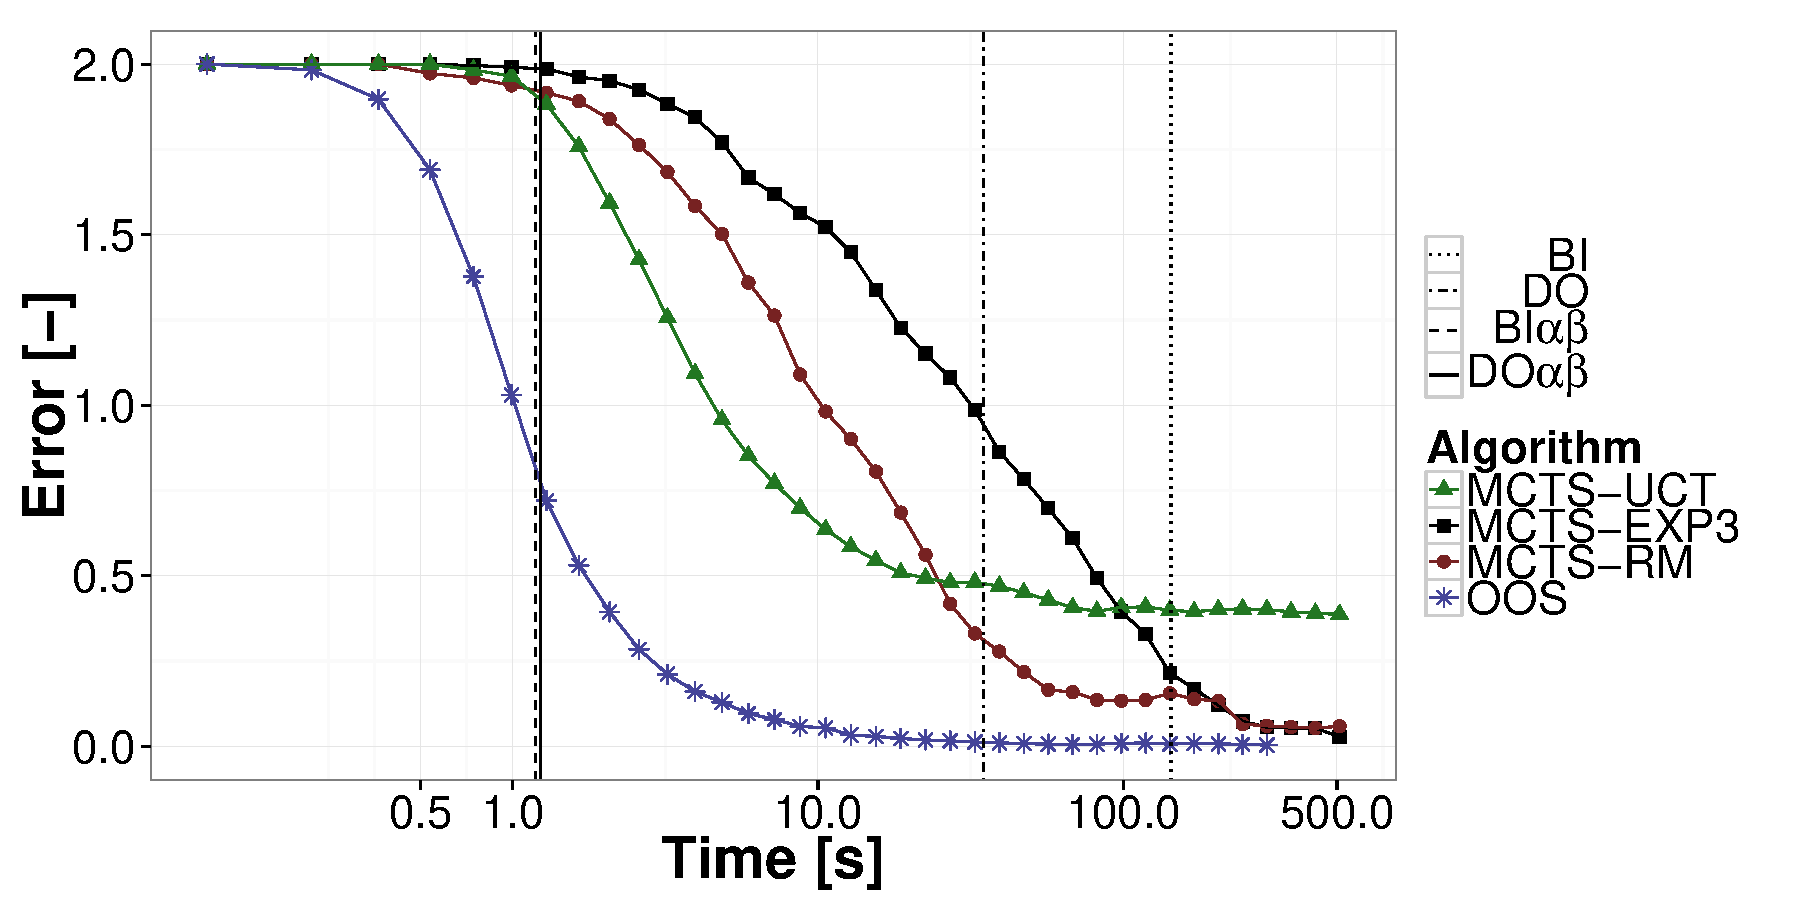
\includegraphics[width=0.85\textwidth]{figures/convergence-tron.pdf}
\caption{Convergence comparison of different sampling algorithms on Tron on grid $5\times6$. The vertical lines correspond to computation times for exact algorithms.} \label{fig:off:conv:tron}
\end{figure}


\subsection{Online Search}

This sections compares the performance of all the algorithms in head-to-head matches in large instances of the same games as we used in equilibrium computation experiments. Each algorithm has a strictly limited computational time per move set to one or five seconds. After this time, it has to output an action to be played in the current game state and afterwards, it is informed about the action selected by its opponent. The game proceeds to the following state and the algorithm have additional time for computation. As described in Section~\ref{sec:online}, all algorithms keep results of previous computations and do not start form scratch in the following move. 
We use only $\doab$ as a representative of backward induction algorithms in this comparison, because it was clearly the fastest algorithm in all the considered games and it provides practically the same solution with a fixed search depth.
In the following experiments, we aim to identify the algorithms that are most suitable in the online search setting and study the relation of the performance in approximating the equilibrium in the offline setting and actual game playing performance in the matches. In this section, we report mainly the win-rates of the algorithms, in which a tie is counted as half win.
The results are mean of at least 1000 matches with half of 95\% confidence interval in brackets. The parameters of the algorithms are initially hand tuned to OOS:0.6,UCT:2,EXP3:0.2,RM:0.1. We discuss the influence of the parameters in Section~\ref{sec:eval:online:tuning}.

\subsubsection{Goofspiel}
\begin{figure}
\centering
\begin{scriptsize}
\begin{tabular}{|r|rrrrrr|}\hline
1s&DOAB&OOS&UCT&EXP3&RM&RAND\\\hline
DOAB&49.0(3.0)&49.6(3.0)&37.1(2.0)&24.0(1.8)&28.2(1.9)&88.7(1.3)\\
OOS&52.9(3.0)&48.5(3.0)&45.9(3.0)&42.1(2.9)&42.3(2.9)&73.8(2.6)\\
UCT&62.4(2.9)&53.9(3.0)&48.3(3.0)&50.6(2.9)&50.7(2.9)&66.3(2.8)\\
EXP3&76.3(2.5)&57.5(2.9)&48.3(2.9)&51.4(2.4)&42.9(2.6)&66.3(2.8)\\
RM&71.6(2.7)&57.8(2.9)&49.0(2.9)&56.1(2.6)&50.0(2.9)&66.2(2.8)\\
RAND&8.6(1.7)&26.2(2.6)&34.3(2.8)&29.1(2.7)&35.0(2.8)&49.6(3.1)\\
\hline
\end{tabular}
\begin{tabular}{|r|rrrrrr|}\hline
5s&DOAB&OOS&UCT&EXP3&RM&RAND\\\hline
DOAB&49.5(3.2)&35.1(3.0)&25.5(2.8)&13.8(2.2)&18.9(2.5)&91.2(1.8)\\
OOS&61.2(3.1)&51.8(3.2)&47.9(3.2)&42.1(3.1)&47.2(3.2)&70.9(2.9)\\
UCT&71.4(2.9)&52.8(3.2)&50.1(3.2)&52.9(3.1)&49.7(3.2)&61.3(3.1)\\
EXP3&85.2(2.2)&59.2(3.1)&45.8(3.1)&50.9(1.5)&46.9(2.5)&65.6(3.0)\\
RM&78.5(2.6)&56.8(3.1)&48.2(3.1)&55.0(2.5)&51.2(2.8)&62.6(3.1)\\
RAND&8.2(1.8)&28.1(2.9)&39.0(3.1)&30.5(2.9)&37.7(3.1)&51.1(3.2)\\
\hline
\end{tabular}

\begin{tabular}{|r|rrrrrr|}\hline
* 1s&DOAB&OOS&UCT&EXP3&RM&RAND\\\hline
DOAB&49.5(1.2)&18.0(1.0)&14.5(0.8)&8.9(0.6)&10.5(0.7)&62.1(1.1)\\
OOS&82.3(1.0)&48.6(1.4)&47.2(1.3)&44.3(1.3)&42.0(1.3)&80.4(1.0)\\
UCT&87.4(0.9)&53.8(1.3)&50.6(1.4)&48.7(1.3)&45.9(1.3)&80.0(1.0)\\
EXP3&92.6(0.7)&55.7(1.3)&50.6(1.3)&50.3(1.3)&45.2(1.2)&83.5(0.9)\\
RM&91.5(0.7)&58.8(1.3)&54.7(1.3)&54.7(1.2)&49.7(1.3)&83.6(0.9)\\
RAND&37.4(1.2)&19.2(1.0)&19.9(1.0)&16.1(0.9)&16.3(0.9)&49.8(1.4)\\
\hline
\end{tabular}

\end{scriptsize}
\caption{Win-rate in head-to-head matches of Goofspiel(13) with decreasing nature cards with one (top) and five (middle) seconds per move. (bottom) Win-rate in Goofspiel(13) and known random sequences of nature cards.}\label{fig:matches:goof}
\end{figure}

In head-to-head comparison, we use Goofspiel with 13 cards, as it is played by humans. However, for the sake of consistency with the offline results, we assume a fixed known sequence of the cards of the nature player. The game has still more than $3.8\times 10^{19}$ leaf nodes. The results are presented in Figure~\ref{fig:matches:goof}.

The first two tables presents the results for decreasing sequence of nature player's cards. Even though $\doab$ uses a domain-specific evaluation function, it does not win significantly against any of the sampling algorithms not using any domain knowledge with one second per move. It tied with OOS and it lost by the largest margin to the MCTS-Exp3. With five seconds per move, even OOS is winning against $\doab$ with MCTS-Exp3 still being its strongest opponent. The same conclusions can be drawn from the experiments with fixed random ordering of the nature players presented in the third table labelled by ``*''.


The differences in the performance of sampling algorithms are relatively small. Even though OOS converges the fastest in the offline experiment (see Figure~\ref{fig:off:conv:gs}), it is losing against all other algorithms with 1 second per move. Its performance improves with 5 seconds per move, but it still does not significantly outperform any other sampling algorithm. With both time settings, RM seems to perform slightly the best. Its performance against other algorithms is very similar to Exp3, but it significantly wins in their mutual matches.

\subsubsection{Oshi-Zumo}
\begin{figure}[t!]
\centering
\begin{scriptsize}
\begin{tabular}{|r|rrrrrr|}\hline
1s&DOAB&OOS&UCT&EXP3&RM&RAND\\\hline
DOAB&50.0(0.0)&91.1(1.2)&89.1(1.3)&89.2(1.3)&85.1(1.5)&98.8(0.5)\\
OOS&12.9(1.4)&53.5(3.0)&52.0(2.1)&56.9(2.0)&31.4(1.9)&97.3(0.7)\\
UCT&11.7(1.4)&53.8(2.1)&50.5(3.0)&55.3(2.1)&32.3(1.9)&94.0(1.0)\\
EXP3&11.1(1.3)&47.3(2.1)&45.1(2.1)&48.9(3.0)&26.0(1.8)&94.2(0.9)\\
RM&13.8(1.5)&73.1(1.8)&67.8(1.9)&75.5(1.8)&48.1(3.0)&99.0(0.4)\\
RAND&1.3(0.5)&3.4(0.7)&5.6(1.0)&5.3(0.9)&0.7(0.3)&48.5(2.9)\\
\hline
\end{tabular}
\begin{tabular}{|r|rrrrrr|}\hline
5s&DOAB&OOS&UCT&EXP3&RM&RAND\\\hline
DOAB&49.6(1.4)&93.2(1.5)&92.1(1.7)&91.2(1.7)&89.6(1.9)&99.1(0.6)\\
OOS&11.6(2.0)&54.9(2.9)&51.3(3.0)&50.0(3.0)&34.9(2.8)&98.2(0.8)\\
UCT&8.9(1.8)&54.1(3.0)&51.2(3.0)&51.1(3.0)&35.0(2.8)&97.2(1.0)\\
EXP3&9.0(1.8)&53.5(3.0)&46.9(3.0)&50.6(2.9)&31.6(2.8)&97.9(0.9)\\
RM&10.1(1.8)&72.0(2.6)&64.5(2.9)&69.2(2.7)&51.5(2.9)&99.9(0.1)\\
RAND&0.8(0.6)&3.2(1.1)&3.6(1.1)&1.6(0.8)&1.0(0.6)&49.6(2.9)\\
\hline
\end{tabular}
\begin{tabular}{|r|rrrrrr|}\hline
E 1s&DOAB&OOS&UCT&EXP3&RM&RAND\\\hline
DOAB&50.0(0.0)&83.2(2.3)&28.8(2.8)&66.1(2.9)&56.8(3.0)&98.8(0.7)\\
OOS&33.8(2.9)&59.5(2.9)&30.9(2.8)&40.0(3.0)&29.4(2.7)&96.6(1.1)\\
UCT&69.8(2.8)&80.9(2.4)&46.5(3.0)&74.8(2.6)&62.0(3.0)&97.8(0.9)\\
EXP3&30.3(2.8)&63.9(2.9)&25.2(2.6)&52.7(3.0)&43.7(3.0)&96.2(1.2)\\
RM&42.2(3.0)&80.5(2.4)&43.2(3.0)&56.9(3.0)&48.7(3.0)&99.2(0.5)\\
RAND&1.4(0.7)&3.0(1.0)&2.6(1.0)&4.6(1.2)&0.5(0.4)&49.0(2.9)\\
\hline
\end{tabular}
\begin{tabular}{|r|rrrrrr|}\hline
E 5s&DOAB&OOS&UCT&EXP3&RM&RAND\\\hline
DOAB&49.4(1.3)&83.0(2.4)&16.1(2.3)&38.1(3.2)&66.1(3.1)&98.9(0.7)\\
OOS&32.8(3.0)&59.3(3.1)&28.3(2.9)&27.4(2.9)&33.3(3.0)&98.3(0.8)\\
UCT&82.7(2.4)&83.5(2.4)&49.2(3.2)&65.0(3.1)&65.5(3.1)&99.1(0.6)\\
EXP3&58.7(3.2)&78.0(2.7)&32.7(3.0)&47.3(3.2)&64.3(3.1)&99.2(0.5)\\
RM&35.4(3.1)&77.1(2.6)&31.5(3.0)&35.4(3.1)&45.8(3.1)&99.2(0.6)\\
RAND&1.0(0.7)&1.8(0.9)&2.0(0.9)&1.9(0.9)&0.5(0.4)&49.9(3.0)\\
\hline
\end{tabular}

\end{scriptsize}
\caption{Win-rate in head-to-head matches of Oshi-Zumo(50,3,1). From top down first 1 and 5 seconds per move without evaluation function, then the same with evaluation function used in sampling algorithms (denoted by ``E'').}\label{fig:matches:oz}
\end{figure}

In Oshi-Zumo, we use the setting with 50 coins, K=3 fields on each side of the board and minimal bet of 1. We chose this parameters to be consistent with \cite{} and to have a game with larger branching factor.\vlisy{can we estimate game size?}

In this game, the evaluation function used by $\doab$ is much stronger than in Goofspiel and all the sampling algorithms without domain specific knowledge perform poorly against this algorithm (see Figure~\ref{fig:matches:oz}). The loss is even higher with 5 seconds per move. None of the sampling algorithms perform significantly better than the others.

In the offline experiment (Figure~\ref{fig:off:conv:oz}), none of the sampling algorithms was able to converge anywhere close to the equilibirum in short time and the game there was many orders of magnitude smaller. With one second per move, RM is clearly the strongest sampling algorithm, having the strongest opponent among the sampling algorithms in UCT loosing 67.8\% of games. OOS and UCT tie for the second place and Exp3 is the weakest sampling algorithm in this game. With five seconds per move, the differences among the algorithms are a little smaller but the same ranking of the algorithms holds.

Because of high quality of the evaluation function in this game, we allowed the sampling algorithms to use it instead of simulation.
The tables for this variant are labelled OshiE in the figures. With evaluation function, the quality of play of all sampling algorithms is significantly improved. However, $\doab$ still wins over OOS and RM in both time settings.
UCT is clearly the best and Exp3 significantly looses to $\doab$ with one second, but significantly wins with 5 seconds per move.
Superior performance of UCT and Exp3 closely second with 5 seconds, but not 1 second, is obvious also in comparison of the sampling algorithms among each other.\vlisy{Why?}
The main difference between RM, which was the best sampling algorithm without evaluation functions, and the other MCTS algorithms is that RM tries to estimate the quality of each joint action of the players, instead of using a fully decoupled dynamics.
This estimates may be misleading when using the evaluation function.\vlisy{Why?}


\subsubsection{Random Games}
\begin{figure}
\centering
\begin{scriptsize}
\begin{tabular}{|r|rrrrrr|}\hline
1s&DOAB&OOS&UCT&EXP3&RM&RAND\\\hline
DOAB&51.5(2.9)&65.5(2.8)&57.7(2.9)&54.0(2.9)&54.0(2.9)&88.8(1.8)\\
OOS&39.7(2.8)&51.1(2.9)&40.2(2.8)&37.1(2.7)&36.0(2.7)&82.8(2.2)\\
UCT&47.4(2.9)&57.1(2.9)&52.5(2.9)&46.9(2.8)&47.9(2.8)&85.7(2.1)\\
EXP3&48.2(2.8)&65.3(2.7)&54.5(2.9)&49.2(2.9)&51.5(2.9)&91.5(1.6)\\
RM&50.4(2.9)&64.8(2.7)&55.1(2.9)&54.0(2.9)&55.0(2.9)&87.1(1.9)\\
RAND&11.8(1.9)&19.7(2.3)&17.4(2.2)&11.1(1.8)&12.4(1.9)&49.9(2.9)\\
\hline
\end{tabular}
\begin{tabular}{|r|rrrrrr|}\hline
Rand&DOAB&OOS&UCT&EXP3&RM&RAND\\\hline
DOAB&48.7(2.9)&60.5(2.8)&49.4(2.9)&48.6(2.9)&49.8(2.8)&88.0(1.9)\\
OOS&37.1(2.8)&50.9(2.9)&40.2(2.8)&35.8(2.8)&36.1(2.8)&83.1(2.2)\\
UCT&45.5(2.8)&55.3(2.9)&48.9(2.9)&47.8(2.9)&48.9(2.9)&86.9(2.0)\\
EXP3&48.1(2.8)&61.6(2.8)&49.9(2.9)&47.4(2.8)&49.5(2.8)&91.0(1.6)\\
RM&47.2(2.9)&59.9(2.8)&50.5(2.9)&50.9(2.8)&48.4(2.8)&91.2(1.6)\\
RAND&9.9(1.7)&17.1(2.2)&12.2(1.9)&7.6(1.5)&10.1(1.7)&50.1(2.9)\\
\hline
\end{tabular}

\end{scriptsize}
\caption{Win-rate in head-to-head matches of Random games (15,5) with one (top) and five (bottom) seconds per move.}\label{fig:matches:rand}
\end{figure}


The next set of matches was played on 10 different random games with each player having 5 actions in each stage and depth 15. Hence, the game has more than $9.3\times 10^{20}$ leaf nodes. In order to compute the win-rates as in other games, we use signum of the utility value defined in Section~\ref{sec:eval:domains}. The results are presented in Figure~\ref{fig:matches:rand}.

With 1 second per move $\doab$ significantly wins over all other algorithms. With 5 seconds, it already wins only over OOS (in 60.5\% matches), playing tie with the other sampling algorithms. OOS looses also against all MCTS algorithms, which perform practically the same among each other. These performance results are not supported by the speed of convergence in Figure~\ref{fig:off:conv:rg}, where Exp3 converges consistently slower than OOS on the small variant of the game.

\subsubsection{Tron}
\begin{figure}[t!]
\centering
\begin{scriptsize}
\begin{tabular}{|r|rrrrrr|}\hline
1s &DOAB&OOS&UCT&EXP3&RM&RAND\\\hline
DOAB&48.7(0.5)&87.4(1.7)&70.0(2.3)&63.4(2.4)&56.9(2.4)&97.9(0.7)\\
OOS&11.1(1.5)&50.6(2.8)&23.2(2.2)&18.7(2.1)&15.1(1.9)&96.0(1.0)\\
UCT&25.4(2.1)&78.1(2.2)&50.0(2.3)&42.0(2.3)&36.0(2.1)&97.8(0.7)\\
EXP3&28.8(2.2)&80.9(2.2)&55.0(2.3)&49.6(2.3)&43.5(2.3)&97.8(0.7)\\
RM&37.4(2.2)&84.9(2.0)&61.6(2.3)&54.6(2.3)&49.0(2.0)&97.7(0.7)\\
RAND&1.4(0.5)&5.0(1.2)&3.5(0.8)&1.9(0.6)&2.4(0.7)&51.1(3.2)\\
\hline
\end{tabular}
\begin{tabular}{|r|rrrrrr|}\hline
5s&DOAB&OOS&UCT&EXP3&RM&RAND\\\hline
DOAB&51.9(0.8)&90.5(1.5)&76.2(2.2)&64.4(2.5)&62.9(2.3)&98.8(0.5)\\
OOS&10.3(1.5)&50.6(3.0)&27.9(2.3)&23.9(2.3)&19.4(2.0)&93.7(1.2)\\
UCT&20.4(1.9)&69.5(2.3)&46.7(2.7)&43.5(2.4)&35.2(2.3)&97.0(0.8)\\
EXP3&29.8(2.2)&74.3(2.3)&58.4(2.4)&49.8(2.6)&43.5(2.3)&97.3(0.7)\\
RM&32.4(2.0)&80.1(2.0)&62.5(2.3)&58.7(2.2)&50.4(2.5)&97.0(0.7)\\
RAND&1.9(0.6)&6.0(1.2)&3.3(0.8)&2.4(0.7)&3.0(0.7)&49.2(3.3)\\
\hline
\end{tabular}
\begin{tabular}{|r|rrrrrr|}\hline
E 1s&DOAB&OOS&UCT&EXP3&RM&RAND\\\hline
DOAB&46.8(0.9)&63.9(2.1)&54.9(1.5)&53.6(1.9)&46.1(1.8)&98.7(0.5)\\
OOS&37.6(1.8)&49.8(1.9)&45.0(1.4)&44.2(1.6)&40.9(1.4)&96.1(0.9)\\
UCT&45.0(1.5)&56.0(1.8)&50.2(0.5)&44.6(1.1)&43.6(1.2)&97.6(0.7)\\
EXP3&50.1(2.0)&58.2(1.8)&55.0(1.1)&50.9(0.8)&45.1(1.0)&98.2(0.6)\\
RM&51.2(2.0)&62.2(1.7)&55.4(1.2)&54.4(1.0)&49.9(0.4)&97.9(0.6)\\
RAND&2.2(0.7)&3.3(0.9)&2.2(0.7)&0.8(0.4)&1.7(0.6)&49.8(3.0)\\
\hline
\end{tabular}
\begin{tabular}{|r|rrrrrr|}\hline
E 5s&DOAB&OOS&UCT&EXP3&RM&RAND\\\hline
DOAB&50.2(0.3)&66.0(2.3)&51.1(2.0)&45.3(2.3)&42.0(2.1)&98.9(0.5)\\
OOS&40.6(1.8)&52.6(2.3)&43.9(1.7)&44.1(1.7)&40.2(1.8)&95.6(1.1)\\
UCT&50.0(1.8)&56.6(1.9)&50.2(0.7)&48.6(0.9)&45.1(1.3)&97.6(0.7)\\
EXP3&61.2(2.5)&56.2(1.9)&51.1(1.0)&50.6(0.8)&45.9(1.0)&98.6(0.6)\\
RM&58.4(2.2)&62.1(1.9)&55.2(1.1)&54.6(1.0)&49.9(0.7)&98.6(0.6)\\
RAND&3.2(0.8)&5.5(1.3)&2.5(0.8)&1.6(0.6)&1.8(0.7)&47.1(3.3)\\
\hline
\end{tabular}

\end{scriptsize}
\caption{Win-rate in head-to-head matches of Tron $13\time 13$. From top down first 1 and 5 seconds per move without evaluation function, then the same with evaluation function used in sampling algorithms (denoted by ``E'').}\label{fig:matches:tron}
\end{figure}

The large variant of Tron in our evaluation was played on en empty $13\times 13$ board. The branching factor of this game is up to 4 for each player and its depth is up to 83 moves. The results are in Figure~\ref{fig:matches:tron}.

This game also allow for a good evaluation function, hence $\doab$ strongly  outperforms all other algorithms when they do not use the evaluation function. Again, its win-rates are higher with less time per move. RM is its strongest opponent, which is more apparent in the longer time setting, where it looses 37.4\% matches.\vlisy{Check the difference with different player positions!!!}

RM is a clear winner also in the matches among the sampling algorithms with both time settings. With smaller difference among MCTS algorithm with increased computation time, but OOS loosing more to MCTS algorithms with 5 seconds. It won only 15.1\% matches against RM with this setting. UCT performs the worst out of the MCTS algorithms, loosing 61.6\% matches against RM.

As in the case of Oshi Zumo, we also run the matches with the evaluation function used instead of simulation in the MCTS algorithms. The use of evaluation function improves performance of all sampling algorithms, but their final ranking is exactly the opposite in this case. RM is the only algorithm winning over $\doab$ in longer time setting, Exp3 wins only with 1 second and ties with 5 second and UCT ties with 1 second and looses with 5 second per move in 54.9\% of matches. Unlike in the case without knowledge, additional time makes $\doab$ win more often against the opponents with evaluation function. This could be caused by the evaluation function giving more consistent game state quality estimates when it is used in the same depth in the tree. The longer run of MCTS leads to more evaluations in different depths.
Among the sampling algorithms, OOS is the weakest and RM is the strongest in the mutual matches.

\subsubsection{Pursuit-Evasion Game}
\begin{figure}
\centering
\begin{scriptsize}
\begin{tabular}{|r|rrrrrr|}\hline
1s&DOAB&OOS&UCT&EXP3&RM&RAND\\\hline
DOAB&91.7(1.7)&95.2(0.4)&93.1(0.5)&89.0(0.6)&81.8(0.8)&99.6(0.1)\\
OOS&51.8(1.0)&76.6(3.7)&82.0(0.7)&67.6(0.9)&58.3(1.0)&98.1(0.3)\\
UCT&78.7(0.8)&93.1(0.5)&91.9(1.7)&86.5(0.7)&78.0(0.8)&98.8(0.2)\\
EXP3&76.1(0.8)&94.2(0.5)&91.7(0.5)&86.6(2.1)&78.9(0.8)&99.3(0.2)\\
RM&86.1(0.7)&94.9(0.4)&93.4(0.5)&90.2(0.6)&81.3(2.4)&99.2(0.2)\\
RAND&1.9(0.3)&30.7(0.9)&38.1(0.9)&8.0(0.5)&3.9(0.4)&70.9(2.8)\\
\hline
\end{tabular}
\begin{tabular}{|r|rrrrrr|}\hline
5s&DOAB&OOS&UCT&EXP3&RM&RAND\\\hline
DOAB&86.1(2.1)&91.7(1.7)&84.3(2.3)&73.0(2.8)&70.4(2.8)&99.3(0.5)\\
OOS&60.2(3.0)&84.1(2.3)&76.2(2.6)&57.3(3.1)&58.8(3.1)&98.5(0.8)\\
UCT&87.5(2.0)&93.2(1.6)&85.4(2.2)&79.9(2.5)&75.3(2.7)&99.0(0.6)\\
EXP3&85.3(2.2)&95.0(1.4)&85.9(2.2)&78.8(2.5)&76.2(2.6)&99.7(0.3)\\
RM&90.0(1.9)&94.9(1.4)&87.1(2.1)&78.5(2.5)&75.2(2.7)&99.2(0.6)\\
RAND&3.1(1.1)&28.3(2.8)&30.8(2.9)&1.6(0.8)&1.5(0.8)&71.0(2.8)\\
\hline
\end{tabular}

\end{scriptsize}
\caption{Win-rate in head-to-head matches of Pursuit evasion game with time limit of 15 moves and $10\times 10$ grod board. One (top) and five (bottom) seconds per move.}\label{fig:matches:peg}
\end{figure}



The last game we use in this part of evaluation is the pursuit-evasion game on empty $10\times 10$ grid with $15$ moves time limit and 10 different randomly selected initial positions of the units. The branching factor is up to 12, causing the number of leaf nodes to be less than $10^16$.

The results in Figure~\ref{fig:matches:peg} show that the game is strongly biased towards the first player, which is the evader. The self-play results on the diagonal shows that $\doab$ won over 91\% matches against itself as the evader. Adding more computational time improved the play of the pursuer in self-play for all algorithms besides OOS. With one second per move, $\doab$ and EM tied for the first place, but with 5 seconds per move, RM without any domain knowledge already performs better than $\doab$ against each of the opponents, while having statistically significant difference of performance only against Exp3, against which $\doab$ on the first position wins 73\% of matches and RM wins 78.5\% of matches. The other two MCTS variants have similar performance in both time settings and OOS is consistently the weakest. 
These results are consistent with the offline convergence results in Figure~\ref{fig:off:conv:peg}, in which in short time, RM converges significantly the fastest.

\subsubsection{Parameter tuning}\label{sec:eval:online:tuning}

\begin{figure}
\centering
\begin{scriptsize}
\begin{tabular}{|r|rrrrrr|}\hline
Time&\multicolumn{6}{|c|}{OOS}\\
&\textbf{0.6}&0.5&0.4&0.3&0.2&0.1\\
1s&12.9(1.4)&12.5(4.6)&18.0(5.2)&12.0(4.5)&13.5(4.7)&17.5(5.2)\\
5s&10.9(1.4)&8.3(3.1)&14.2(3.9)&10.2(3.4)&14.0(3.9)&14.2(3.9)\\\hline
&\multicolumn{6}{|c|}{UCT}\\
&4&\textbf{2}&1.5&1&0.8&0.6\\
1s&11.2(3.5)&11.7(1.4)&16.5(4.2)&13.8(3.8)&15.8(4.1)&11.8(3.6)\\
5s&7.3(2.9)&11.3(1.4)&8.7(3.2)&6.3(2.7)&8.2(3.1)&10.5(3.4)\\\hline
&\multicolumn{6}{|c|}{EXP3}\\
&0.6&0.5&0.4&0.3&\textbf{0.2}&0.1\\
1s&24.5(4.8)&24.0(4.8)&16.0(4.1)&18.2(4.3)&11.1(1.3)&7.0(2.9)\\
5s&16.7(4.2)&15.8(4.1)&10.2(3.4)&11.2(3.5)&11.0(1.3)&5.7(2.6)\\\hline
&\multicolumn{6}{|c|}{RM}\\
&0.75&0.5&0.3&0.2&\textbf{0.1}&0.05\\
1s&18.0(4.3)&26.7(4.9)&21.0(4.6)&11.5(4.3)&13.8(1.5)&12.3(3.7)\\
5s&17.5(5.2)&15.0(7.0)&13.0(5.3)&11.5(6.2)&14.4(1.5)&16.0(5.0)\\\hline
\end{tabular}

\end{scriptsize}
\caption{The win-rate of different algorithms against $\doab$ in Oshi Zumo. The bold parameter value is used in the head-to-head performance evaluation above.}\label{fig:tuning}
\end{figure}

The exploration parameters for the sampling algorithms in the complete head-to-head comparison above were hand-tuned and fixed to 0.6 for OOS, 2 for UCT, 0.2 for Exp3 and 0.1 for RM. In Figure~\ref{fig:tuning}, we evaluate how the performance of the algorithms can be improved by tuning the parameters for a specific game. We chose the Oshi-Zumo game, in which all the sampling algorithms performed the worst and we tuned their exploration parameter against their strongest opponent -- $\doab$. We chose this worst case, because in zero-sum games, the optimal player that approximates the Nash equilibrium in the game should maximize its performance against its strongest opponent.\vlisy{It would be good to add more samples here.}

The influence of the exploration parameter in OOS is not statistically significant after 300 matches played for this table. The differences with 5 seconds per move were even smaller. While the default parameter is likely not optimal in this setting, it is still meaningful.
The performance of UCT can likely be slightly improved by setting the parameter to 1.5 instead of 2 for the shorter time setting, but our default value seems to be optimal for the longer time setting. Still, none of the differences is statistically significant with 95\% probability.
Setting much higher exploration for Exp3 can significantly improve the performance of the algorithm against $\doab$ with one second per move, but the influence of the parameter is weaker with the longer time setting. Running some of the matches with higher exploration against the other algorithms showed then while it slightly improves the performance against $\doab$, it makes the performance of the algorithm against other sampling methods worse.
Even EM algorithm can be improved by increased exploration in this setting. Again, with stronger influence in shorter time settings. 

While tuning the parameters can have influence on game playing performance against specific opponents in specific games, none of the parameter settings could help the algorithms perform anywhere close to $\doab$ in this game. This shows that with a strong evaluation function, backward induction algorithm clearly outperforms the sampling algorithms without domain specific knowledge.

\subsubsection{Summary}

\vlisy{possibly move to some general discussion}

Several conclusions can be made form the head-to-head comparison of the algorithms in larger games. 
First, the fast convergence and low exploitability of OOS algorithm in the smaller variants of the games is not very good predictor of its performance in the online setting. OOS was consistently one of the worst performing algorithm. 
Second, while $\doab$ with a good evaluation function wins over the sampling algorithms without domain specific knowledge, it is not necessary the case with a weaker evaluation function, as we can see in Goofspiel, and if even the sampling algorithms are allowed to use the evaluation functions, $\doab$ is already outperform by either RM in Tron or UCT in Oshi-Zumo. Evaluation function improves the performance of OOS the least of all sampling algorithms.
Third, with longer thinking time, the differences between win-rates of the sampling algorithms are getting smaller. Longer thinking time has also the same effect in the parameter tuning and it also significantly improves the performance of the sampling algorithms against backward induction.
Finally, RM seems to be consistently the best performing algorithm in game playing for this class of games. Out of all the games and both time settings, it looses only in Oshi-Zumo with evaluation function, where it is outperformed by UCT.

%Discussion: 
%-low exploitability not necessary correlated to quality of play, possibly other solution concept, such as non-dominated strategies.
%-sampling algorihtms perform better compared to $\doab$ and coloser to each other with more time per move
%- evaluatin functions help, but they help OOS less
%- OOS did not proove to be good even though it converges the fastest
%- RM is very consistently the overall winner with UCT to consider with evaluation function
%- more time causes less sensitivity to parameters
